\newif\ifshowsolutions
\showsolutionsfalse
\documentclass{article}
\usepackage{listings}
\usepackage{amsmath}
\usepackage{subfigure}
\usepackage{subfig}
\usepackage{bbm}
\usepackage{amsthm}
\usepackage{amsmath}
\usepackage{amssymb}
\usepackage{graphicx}
\usepackage{mdwlist}
\usepackage[colorlinks=true]{hyperref}
\usepackage{geometry}
\usepackage{titlesec}
\geometry{margin=1in}
\geometry{headheight=2in}
\geometry{top=2in}
\usepackage{palatino}
\usepackage{mathrsfs}
\usepackage{fancyhdr}
\usepackage{paralist}
\usepackage{todonotes}
\setlength{\marginparwidth}{2.15cm}
\usepackage{tikz}
\usetikzlibrary{positioning,shapes,backgrounds}
\usepackage{float} % Place figures where you ACTUALLY want it
\usepackage{comment} % a hack to toggle sections
\usepackage{ifthen}
\usepackage{mdframed}
\usepackage{verbatim}
\usepackage[strings]{underscore}
\usepackage{listings}
\usepackage{bbm}
\usepackage{bm}
\usepackage{algorithm}
\usepackage{algpseudocode}
\usepackage{mathtools}
\rhead{}
\lhead{}

\renewcommand{\baselinestretch}{1.15}

% Shortcuts for commonly used operators
\newcommand{\E}{\mathbb{E}}
\newcommand{\Var}{\operatorname{Var}}
\newcommand{\Cov}{\operatorname{Cov}}
\newcommand{\Bias}{\operatorname{Bias}}
\DeclareMathOperator{\argmin}{arg\,min}
\DeclareMathOperator{\argmax}{arg\,max}
\DeclareMathOperator{\arginf}{arg\,inf}
\DeclareMathOperator{\argsup}{arg\,sup}

% do not number subsection and below
\setcounter{secnumdepth}{1}

% custom format subsection
\titleformat*{\subsection}{\large\bfseries}

% set up the \question shortcut
\newcounter{question}[section]
\newenvironment{question}[1][]
  {\refstepcounter{question}\par\addvspace{1em}\textbf{Question~\Alph{question}\!
    \ifthenelse{\equal{#1}{}}{}{ [#1 points]}: }}
    {\par\vspace{\baselineskip}}

\newcounter{subquestion}[question]
\newenvironment{subquestion}[1][]
  {\refstepcounter{subquestion}\par\medskip\textbf{\roman{subquestion}.\!
    \ifthenelse{\equal{#1}{}}{}{ [#1 points]:}} }
  {\par\addvspace{\baselineskip}}

\titlespacing\section{0pt}{12pt plus 2pt minus 2pt}{0pt plus 2pt minus 2pt}
\titlespacing\subsection{0pt}{12pt plus 4pt minus 2pt}{0pt plus 2pt minus 2pt}
\titlespacing\subsubsection{0pt}{12pt plus 4pt minus 2pt}{0pt plus 2pt minus 2pt}


\newenvironment{hint}[1][]
  {\begin{em}\textbf{Hint: }}{\end{em}}


\chead{%
  {\vbox{%
      \vspace{2mm}
      \large
      Mass-friction\hfill
      Adjoint vs. Naive Gaussian \hfill \\[1pt]
      Rate-and-state friction\hfill
      January 10th, 2023
    }
  }
}
\newcommand{\la}{\left\langle}
\newcommand{\ra}{\right\rangle}
\newcommand{\indep}{\raisebox{0.05em}{\rotatebox[origin=c]{90}{$\models$}}}
\begin{document}
\pagestyle{fancy}
\section{Problem setup}
We consider a simple mass-block sliding on a horizontal surface driven by a spring moving at constant rate $V$, 
where the friction in between is rate-and-state dependent. 

\begin{figure}[H]
    \centering
    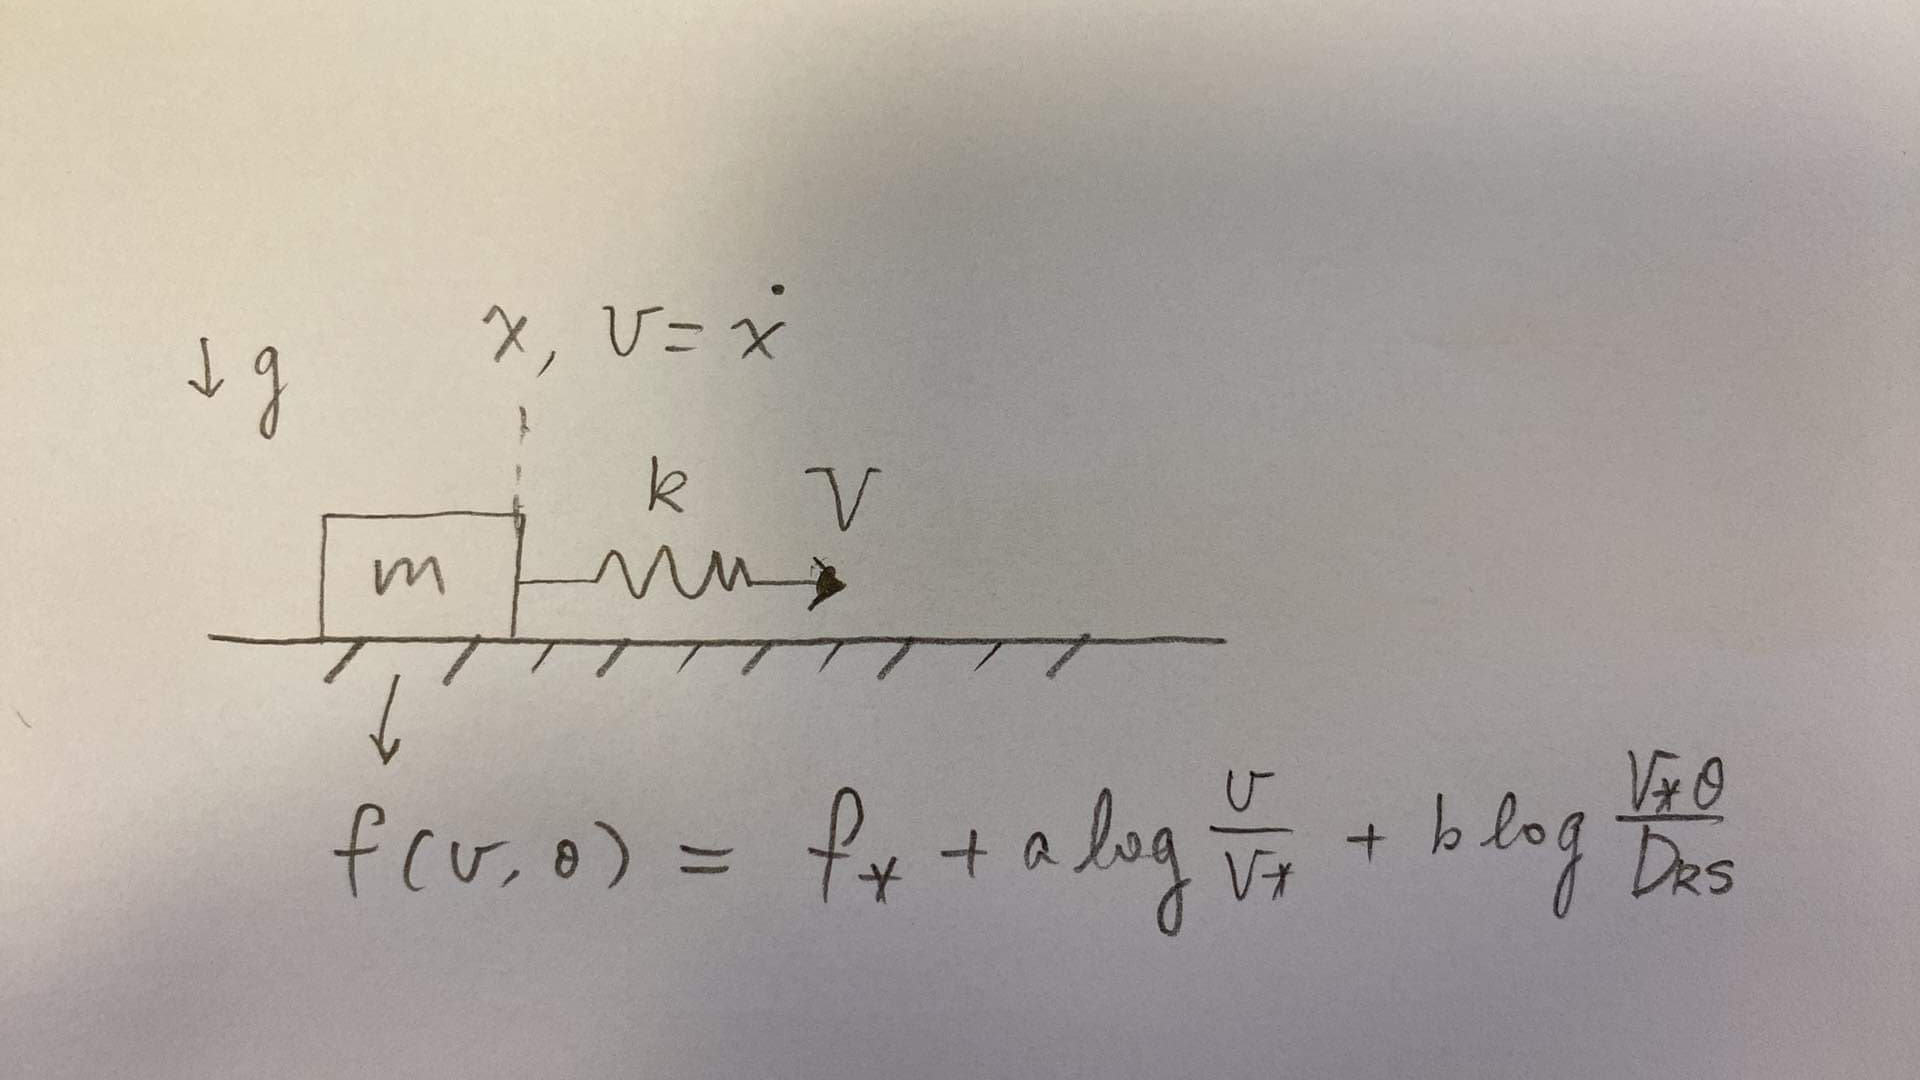
\includegraphics[width=0.8\textwidth]{shit1.png}
    \caption{Schematic figure of mass block sliding on a frictional surface}
    \label{fig:massBlockSliding}
\end{figure}

The parameters used: 
\begin{itemize}
    \item $k$: Stiffness of the spring
    \item $m$: Mass of the sliding block
    \item $V$: Constant speed at which the spring is being pulled
    \item $g$: Gravitational acceleration
    \item $x$: Position of the mass block
    \item $v$: Velocity of the mass block
    \item $\theta$: State variable
    \item $f(v=\dot{x}, \theta)$: Friction coefficient
    \item $t$: Time, within $[0, T]$
\end{itemize}

The equation of motion can be written as 
\begin{align}
    m\Ddot{x} + k(x - x_p) - mg\left[f_* + a\log(\dot{x}/V_*) + b \log(V_* \theta / D_{RS})\right] &= 0 \label{eq:motion}\\
    \dot{\theta} - (1 - \dot{x} \theta / D_{RS}) &= 0 \label{eq:evolutionAging}
\end{align}

The system has two generalized coordinates, 
\begin{align}
    \boldsymbol{q} &= [x, \theta]^T \label{eq:GenCoords}. 
\end{align}
We define inertia potential $E^{\text{in}}(\boldsymbol{q})$, 
elastic potential
$E(\boldsymbol{q})$ and 
dissipation potential $D(\boldsymbol{\dot{q}}, \boldsymbol{q})$ such that
\begin{align}
    \nabla_{\boldsymbol{q}} \left[E^{\text{in}}(\boldsymbol{q}) + E(\boldsymbol{q})\right] + \nabla_{\dot{\boldsymbol{q}}}D(\boldsymbol{\dot{q}}, \boldsymbol{q}_n) = 0 \label{eq:GenGradZero}
\end{align}
gives us (\ref{eq:motion}) and (\ref{eq:evolutionAging}).
\textbf{Note} that $\boldsymbol{q}_n$ and $\boldsymbol{q}_{n-1}$ are already known from previous time steps, 
and thus (\ref{eq:GenGradZero}) is not fully implicit, 
since the $D(\boldsymbol{\dot{q}}, \boldsymbol{q})$ has its second argument evaluated at the previous time step. 

Writing the potentials in terms of $\boldsymbol{q} = [x, \theta]^T$, 
if we define 

\begin{align}
    E^{\text{in}}(x, \theta) &= \frac{m}{2} \left(\frac{x - 2x_n+x_{n-1}}{\Delta t}\right)^2 \label{eq:Ein}\\
    E(x, \theta) &= \frac{k}{2}(x_p - x)^2 + \frac{\Delta t}{2} \left(\frac{\theta - \theta_n}{\Delta t}\right)^2 \label{eq:Eelastic}, 
\end{align}

\noindent then if we are able to find $D(\dot{x}, \dot{\theta}; x_n, \theta_n)$ such that 
\begin{align}
    \frac{\partial D}{\partial \dot{x}} &= -mg\left[f_* + a\log(\dot{x}/V_*) + b \log(V_* \theta_n / D_{RS})\right] \label{eq:proposeddDdx} \\
    \frac{\partial D}{\partial \dot{\theta}} &= - (1 - \dot{x} \theta_n / D_{RS}) \label{eq:proposeddDdTheta}, 
\end{align}
(\ref{eq:GenGradZero}) would be equivalent as am optimization problem:
\begin{align}
    \boldsymbol{q}_{n+1} &= \argmin_{\boldsymbol{q}} \left\{E^{\text{in}}(\boldsymbol{q}) + E(\boldsymbol{q}) + \Delta t D\left(\frac{\boldsymbol{q}-\boldsymbol{q}_n}{\Delta t}, \boldsymbol{q}_n\right)\right\} \label{eq:OptProb}. 
\end{align}
Actually now there is already an obviously problem, 
since $D$ is a relatively-smooth function of $\dot{x}, \dot{\theta}$, 
if you take a partial derivative of (\ref{eq:proposeddDdx}) w.r.t $\dot{\theta}$, 
and (\ref{eq:proposeddDdTheta}) w.r.t $\dot{x}$, 
you already can see that such a $D$ cannot exist unless $\theta_n$ is always $0$. 

But anyways, 
here's another argument, 
assuming such a $D(\dot{x}, \dot{\theta}; x_n, \theta_n)$ exists, 
starting from (\ref{eq:proposeddDdTheta}), 
we would have 
\begin{align}
    D(\dot{x}, \dot{\theta}) = -\dot{\theta} + \frac{\theta_n}{D_{RS}} \dot{x}\dot{\theta} + F_1(\dot{x}) \label{eq:DefF1}, 
\end{align}
plugging back into (\ref{eq:proposeddDdx}), 
we have a \textbf{problem of inconsistency}:
\begin{align}
    \frac{\theta_n}{D_{RS}} \dot{\theta} + F_1'(\dot{x}) &= \frac{\partial D}{\partial \dot{x}} = -mg\left[f_* + a\log(\dot{x}/V_*) + b \log(V_* \theta_n / D_{RS})\right] \label{eq:InconsProb}, 
\end{align}
where the right hand side only depends on $\dot{x}$, 
but the left hand side decisively has $\dot{\theta}$. 

This seems to mean that an additional term is needed in the rate-and-state friction formulation 
\begin{align*}
    f(\dot{x}, \theta) &= f_* + a\log(\dot{x}/V_*) + b\log(V_*\theta / D_{RS}). 
\end{align*}

% Using Neural Network to find potentials
\newpage
\section{Using Neural network to find potentials for Rate and State friction}
\subsection{Taking $F_{fric}(\dot{x}, \xi)=\frac{\partial W}{\partial x}(x) + \frac{\partial D^\dagger}{\partial \dot{x}}(\dot{x}, \xi)$}
Here instead we assume the friction $F_{fric}$ at time $t$ given sliding history $x(t), t \in [0, t]$ is the solution of the following ODE system:
\begin{align}
    F_{fric}(\dot{x}, \boldsymbol{\xi}) &= \frac{\partial W}{\partial x}(x) + \frac{\partial D^\dagger}{\partial \dot{x}}(\dot{x}, \bm{\xi}) \label{eq:potentialWDDotX}\\
    \frac{d D}{d \dot{\boldsymbol{\xi}}} + \frac{\partial D^\dagger}{\partial \boldsymbol{\xi}} &= 0 \label{eq:potentialDDotX}, 
\end{align}
where $W = W(x), D^\dagger = D^\dagger(\dot{x}, \boldsymbol{\xi}), D = D(\dot{\boldsymbol{\xi}})$, 
$x$ is the displacement, $\dot{x}$ is the slip rate, and 
$\bm{\xi} \in \mathbb{R}^d$ is the state variable vector. 
Then the equilibrium equation in (\ref{eq:motion}):
\begin{align*}
    F^{inertia}(x) + F^{spring}(x) + F^{fric}(\dot{x}, \bm{\xi}) = 0
\end{align*}
can be written as 
\begin{align}
    \frac{\partial E^{inertia}}{\partial x}(x) + \frac{\partial E^{spring}}{\partial x}(x) 
    + \frac{\partial W}{\partial x} (x) 
    + \frac{\partial D^\dagger}{\partial \dot{x}}(\dot{x}, \bm{\xi}) = 0 \label{eq:WDPotentialMotionDotX}, 
\end{align}
while the state evolution law is given by the solution of (\ref{eq:potentialDDotX}). 

Then one can show that evolving the solution at time $t_n$ to $t_{n+1}$ can be written as an optimization problem, i.e., 
\begin{align}
    x_{n+1}, \bm{\xi}_{n+1} &= \arginf_{x, \bm{\xi}} \left\{J(x, \xi) \coloneqq E^{in}(x) + E^{sp}(x) + W(x) + \Delta t D^\dagger\left(\frac{x - x_n}{\Delta t}, \bm{\xi}\right) + \Delta t^2 D\left(\frac{\bm{\xi}-\bm{\xi}_n}{\Delta t}\right)\right\},  \label{eq:nToNPlusOneDotX}
\end{align}
where according to our spring-slider model, 
with backward-Euler in the displacement term, 
\begin{align}
    E^{in} (x) &= \frac{m}{2} \left(\frac{x - 2x_n + x_{n-1}}{\Delta t}\right)^2 \\
    E^{sp}(x) &= \frac{k}{2} \left(x - x_p\right)^2
\end{align}
For convexity of $J(x, \xi)$, 
one needs the Hessian to be positive-semi-definite (PSD), 
for the case of $\text{dim}(\xi) = 1$, 
\begin{align*}
    H_J(x, \xi) = \frac{\partial^2 J}{\partial (x, \xi)^2} = 
    \begin{bmatrix}
     J_{xx} & J_{x\xi} \\
     J_{\xi x} & J_{\xi \xi}
    \end{bmatrix}
\end{align*}
\begin{align}
    J_{xx} &= \frac{m}{\Delta t^2} + k + \frac{d^2 W}{d x^2}(x) + \frac{1}{\Delta t} \frac{\partial^2 D^\dagger}{\partial \dot{x}^2}\left(\frac{x - x_n}{\Delta t}, \xi \right) \\
    J_{x\xi} = J_{\xi x} &= \frac{\partial^2 D^\dagger}{\partial \dot{x} \partial \xi} \left(\frac{x - x_n}{\Delta t}, \xi \right) \\
    J_{\xi \xi} &= \Delta t \frac{\partial^2 D^\dagger}{\partial \xi^2} \left(\frac{x - x_n}{\Delta t}, \xi \right) + \frac{d^2 D}{d \dot{\xi}^2}\left(\frac{\xi - \xi_n}{\Delta t}\right). 
\end{align}
For $H_J(x, \xi)$ to be convex, 
all of principal minors needs to be positive-semi-definite, 
i.e., 
\begin{align*}
    J_{xx} &\ge 0 \\
    J_{xx} J_{\xi\xi} - J_{x\xi}^2 &\ge 0, \forall\ x, \xi.
\end{align*}
After re-collecting terms, 
we get that for all $x, \xi, \dot{\xi}$, 
\begin{align}
    2^{-19}&1 \cdot m + \Delta t \left(\frac{\partial^2 D^\dagger}{\partial \dot{x}^2}\right) + \Delta t^2 \left(k + \frac{d^2 W}{dx^2}\right) &\ge 0, \label{eq:PSD1}\\
    & 1 \cdot m \frac{d^2D}{d\dot{\xi}^2} 
    + \Delta t \left(\frac{\partial^2 D^\dagger}{\partial \dot{x}^2} \frac{d^2D}{d\dot{\xi}^2} + m \frac{\partial^2 D^\dagger}{\partial \xi^2}\right) 
    &\notag \\
    & + \Delta t^2 \left[\left(k + \frac{d^2W}{dx^2}\right)\frac{d^2D}{d\dot{\xi}^2} + \frac{\partial^2 D^\dagger}{\partial \dot{x}^2}\frac{\partial^2 D^\dagger}{\partial \xi^2}-\frac{\partial^2D^\dagger}{\partial \dot{x} \partial \xi}\right] 
    &\notag \\
    & + \Delta t^3 \left[\left(k + \frac{d^2W}{dx^2}\right)\frac{\partial^2D^\dagger}{\partial \xi^2}\right] & \ge 0. \label{eq:PSD2}
\end{align}
Note that since we are learning $D^*$, 
which is the Legendre transform of $D(\dot{\xi})$, 
and $D$ is practically computed by the inverse Legendre transform:
\begin{align}
    D(\dot{\xi}) = \sup_{\dot{d}} \left\{\dot{\xi} \dot{d} - D^*\left(\dot{d}\right)\right\}, 
\end{align}
it is always convex. 
Then (\ref{eq:PSD1}, \ref{eq:PSD2}) are always satisfied for small enough $\Delta t$. 

\subsection{Neural Network approximation of potentials}
\noindent Let 
\begin{align*}
    \Tilde{W}(x; w_W) &\approx W(x) \\
    \Tilde{D^\dagger}(\dot{x}, \bm{\xi}; w_{D^\dagger}) &\approx D^\dagger(\dot{x}, \bm{\xi}) \\
    \Tilde{D}^*(\dot{\bm{d}}; w_D) &\approx \sup_{\bm{\dot{\xi}}} \left\{\la \bm{\dot{d}}, \bm{\dot{\xi}} \ra -D(\dot{\bm{\xi}})\right\}
\end{align*}
be the Neural-Network (Multi-layer perceptron) approximation of the proposed potentials $W$ and $D$. 
Given a set of slip-friction history sequences,
\begin{align*}
    \left\{x^{(i)}(\tau), F^{(i)}_{fric}(\tau) : \tau \in [0, T^{(i)}]\right\}_{i \in I}, 
\end{align*}
By solving (\ref{eq:potentialWDDotX}) and (\ref{eq:potentialDDotX}) with $\Tilde{W}, \Tilde{D}^\dagger$ and $\Tilde{D}$, 
one can get $\Tilde{F}_{fric}(\tau;w_W, w_{D^\dagger}, w_D)$, 
and training is done by 
\begin{align}
    w_W^*, w_D^* &= \arginf_{w_W, w_D} \mathbb{E} \left[\|F_{fric}(t) - \Tilde{F}_{fric}(t; w_W, w_D)\|_{\mathcal{L}^p[0, T]}\right] \label{eq:NNPotentialstraining}
\end{align}
The solving algorithm goes like this:
\begin{algorithm}[H]
\caption{Training $\Tilde{W}(x; w_W), \Tilde{D}^\dagger(\dot{x}, \bm{\xi}; w_{D^\dagger})$ and $\Tilde{D}^*(\dot{\bm{d}}; w_D)$}\label{alg:TrainingOneEpoch}
\begin{algorithmic}
%% Setting parameters
% Input space
\Require training sequences $\left\{x^{(i)}(\tau), F^{(i)}_{fric}(\tau) : \tau \in \{t_0, t_1, ..., t_N^{(i)}\}\right\}_{i \in I}$.  
\Require $N_{epochs}$
%% Algorithm begins
\State $iter = 0$
\While{$iter<N_{epochs}$}
    \For {$i \in I$}
        \State Fix $w_W$, $w_{D^\dagger}$, $w_D$
        \For {$n = 1, 2, ..., N^{(i)}$}
            \State $\xi_n \gets \xi_{n-1} + (t_n-t_{n-1}) \dot{\bm{\xi}}_{n-1}$
            \State $\Tilde{F}_{fric, n} \gets \frac{\partial \Tilde{W}}{\partial x_n}(x_n) + \frac{\partial \Tilde{D}^\dagger}{\partial \dot{x}_n}(\dot{x}_n, \bm{\xi}_n)$
            \State \textcolor{red}{$\bm{\dot{\xi}}_n \gets $ solution of $\frac{d \Tilde{D}}{d \dot{\boldsymbol{\xi}}}(\dot{\bm{\xi}}) + \frac{\partial \Tilde{D}^\dagger}{\partial \boldsymbol{\xi}}(\dot{x}_n, \bm{\xi}_n) = 0$}
            \Comment{Actually computes $\dot{\bm{\xi}} = \frac{d \Tilde{D}^*}{d \dot{\bm{d}}}\left(-\frac{\partial \Tilde{D}^\dagger}{\partial \bm{\xi}}\right)$}
        \EndFor
        \State Compute Loss $L(w_W, w_{D^\dagger}, w_D) = \|F_{fric} - \Tilde{F}_{fric}(w_W, w_{D^\dagger}, w_D)\|_{{l}^p}$
        \State Update $w_W, w_{D^\dagger}, w_D$ based on the gradient of $L$ w.r.t. $w_W, w_{D^\dagger}, w_D$
    \EndFor
    \State $iter \gets iter+1$
\EndWhile
\end{algorithmic}
\end{algorithm}

\noindent The issues here are that the red line:
\begin{itemize}
    \item $D(\dot{\bm{\xi}})$ needs to be convex. 
\end{itemize}

\subsection{Formulation without potentials}
\noindent Here instead of training NNs for the potentials, 
we directly train two NNs $F$ and $G$ to approximate
\begin{align}
    F_{fric}(x, \dot{x}, \bm{\xi}) &= F(x, \dot{x}, \bm{\xi}) \label{eq:FFriction} \\
    \dot{\bm{\xi}} &= G(x, \dot{x}, \bm{\xi}) \label{eq:GforXi}, 
\end{align}
and compared the results with the formulation with potentials on two datasets, 
one mimicking the velocity-jump test, 
the other following Burigede's work. 

\newpage
\section{Results}
\noindent We fix the number of training epochs to $100$, 
and use $200$ OpTuna iterations to tune
\begin{itemize}
    \item Number of layers of $\tilde{W}, \tilde{D}^\dagger, \tilde{D}^*$.
    \item Number of Neurons in each layer of $\tilde{W}, \tilde{D}^\dagger, \tilde{D}^*$.
    \item Batch size of training dataset.
    \item The corresponding learning rates.
    \item The $p$ for training loss (we use relative $p$-norm here). 
\end{itemize}
The loss over a dataset is defined as 
\begin{align}
    Loss(p) = \frac{1}{|I|} \sum_{i\in I} \frac{\|f(t)-f_{targ}(t)\|_p}{\|f_{targ}(t)\|_p}, 
\end{align}
and for evaluation of the trained model, 
we use $p=2$ and calculate the loss on a separate test dataset. 

\subsection{Training on VJump vs. Burigede vs. Combined dataset}
The training and testing datasets are generated using the following material parameters:
\begin{align*}
    a &= 0.011 \\
    b &= 0.016 \\
    D_{RS} &= 0.01\ \mathrm{m}\\
    f_* &= 0.58
\end{align*}
And initial condition of 
\begin{align*}
    \theta_0 = 0.01\ \mathrm{s}.
\end{align*}

Here're two tables showing the average $L_2$ error of models trained on VJump training dataset only vs. Burigede training dataset only vs. combination of the two training datasets, 
either combined together or training on one after another. 
\begin{table}[H]
    \centering
    \begin{tabular}{c|cccc}
        \hline
        Test set & VJump (200) & Burigede (200) & Combined_resampled (200) & combined_full (400)\\
        \hline
        VJump & 0.0586 & 0.2962 & 0.1464 & 0.0358\\
        Burigede & 0.0346 & 0.0754 & 0.0455 & 0.0181\\
        \hline
    \end{tabular}
    \caption{Training on combined dataset helps reduce error on either of the original datasets.}
    \label{tab:combinedImprovesPerformance200}
\end{table}
\begin{table}[H]
    \centering
    \begin{tabular}{c|cccc}
        \hline
        Test set & VJump (400) & Continuous (400) & Combined_resampled (400) & combined_full (800)\\
        \hline
        VJump & 0.0317 & 0.2808 & 0.0367 & 0.0206\\
        Continuous & 0.0458 & 0.0705 & 0.0223 & 0.0140\\
        combined & 0.0379 & 0.1702 & 0.0276 & 0.0173\\
        \hline
    \end{tabular}
    \caption{Training on combined dataset helps reduce error on either of the original datasets.}
    \label{tab:combinedImprovesPerformance200}
\end{table}
\begin{table}[H]
    \centering
    \begin{tabular}{c|ccccc}
        \hline
        Test set & combined_full & V_B & B_V & V_B_V & B_V_B\\
        \hline
        VJump & 0.0358 & 0.1566 & 0.2576 & 0.0852 & 0.2912 \\
        Burigede & 0.0181 & 0.0470 & 0.1338 & 0.0440 & 0.0807 \\
        \hline
    \end{tabular}
    \caption{Training on combined dataset vs. B and V datasets one by one.}
    \label{tab:staggeredDoesNotImprovePerformance}
\end{table}
\newpage
\subsubsection{Results on VJump datasets} 
\begin{figure}[H]
    \centering
    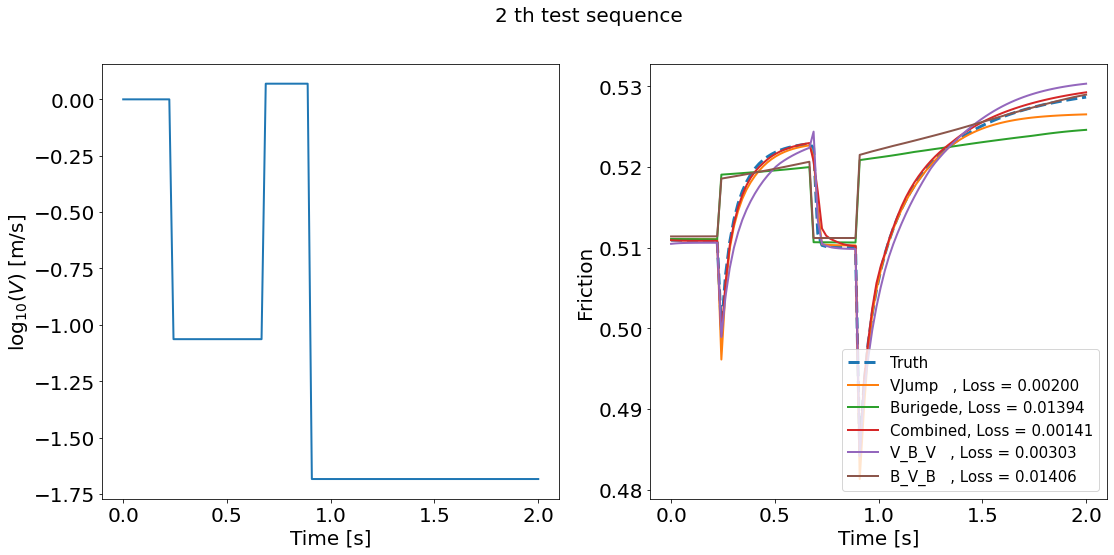
\includegraphics[width=1.0\textwidth]{./images/Trial0112_VJump2.png}
\end{figure}
\begin{figure}[H]
    \centering
    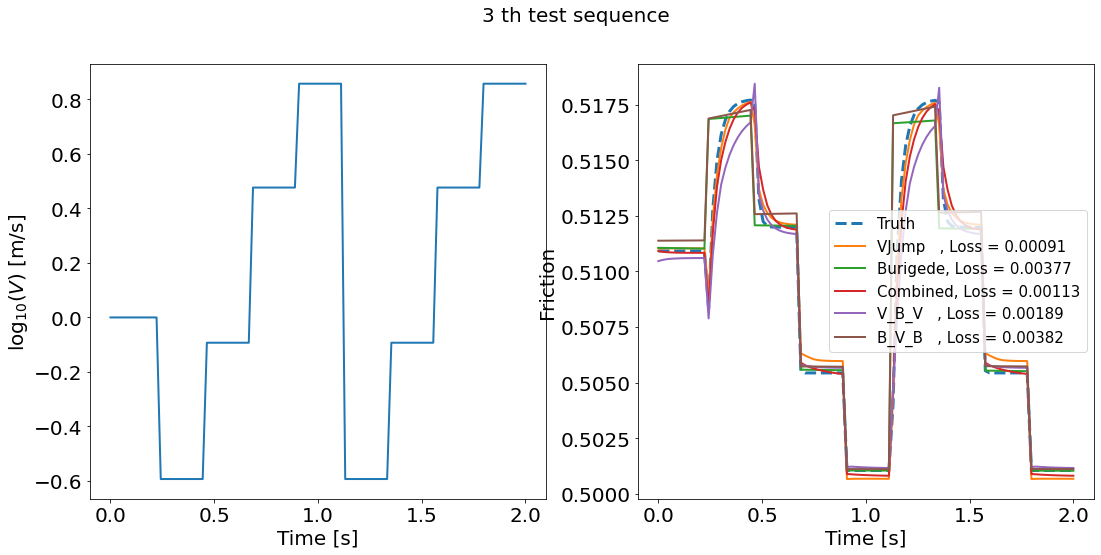
\includegraphics[width=1.0\textwidth]{./images/Trial0112_VJump3.png}
\end{figure}
\begin{figure}[H]
    \centering
    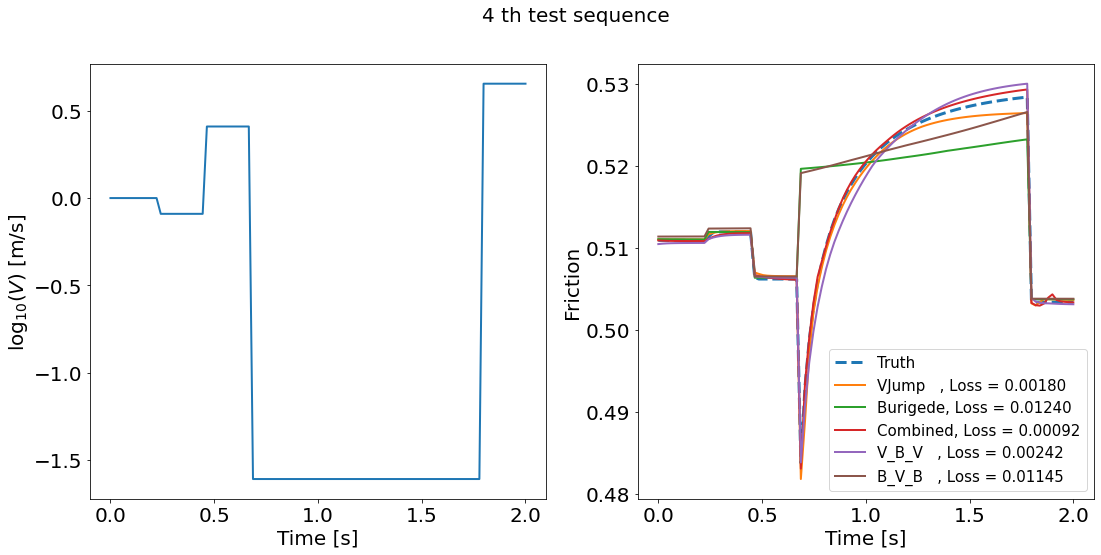
\includegraphics[width=1.0\textwidth]{./images/Trial0112_VJump4.png}
\end{figure}
\begin{figure}[H]
    \centering
    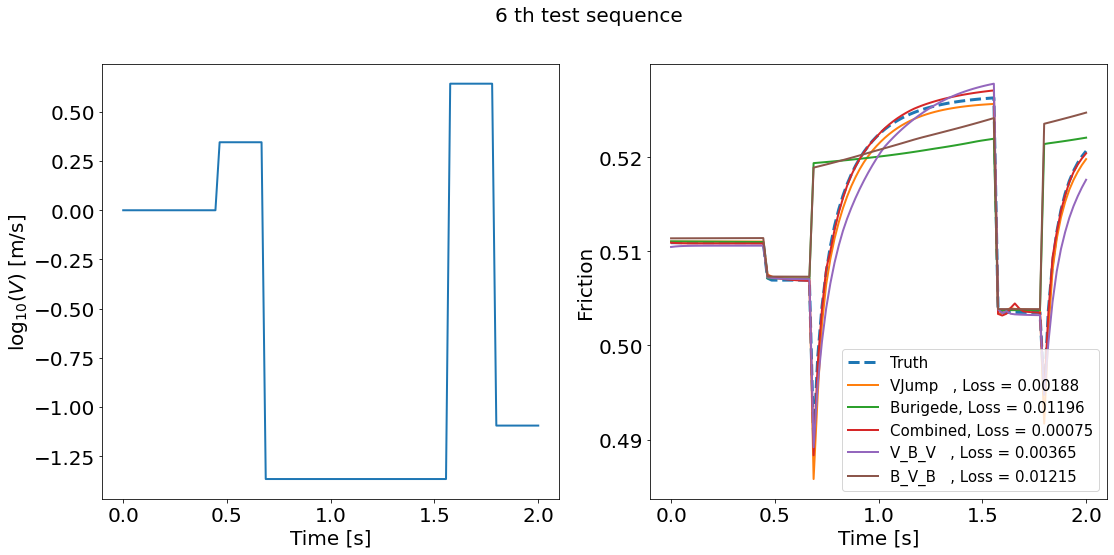
\includegraphics[width=1.0\textwidth]{./images/Trial0112_VJump6.png}
\end{figure}

\newpage
\subsubsection{Results on Burigede datasets}
\begin{figure}[H]
    \centering
    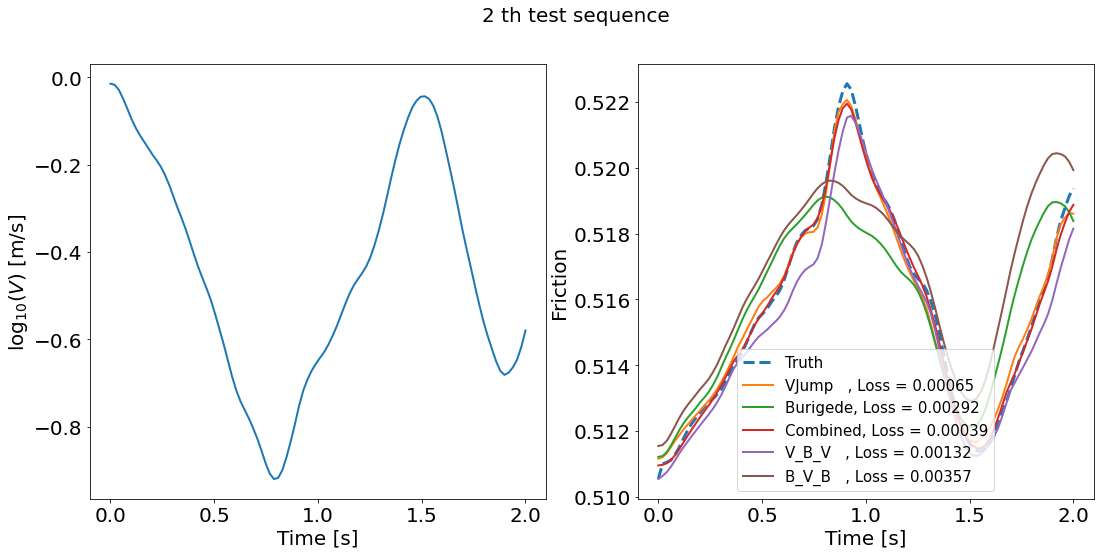
\includegraphics[width=1.0\textwidth]{./images/Trial0112_Burigede2.png}
\end{figure}
\begin{figure}[H]
    \centering
    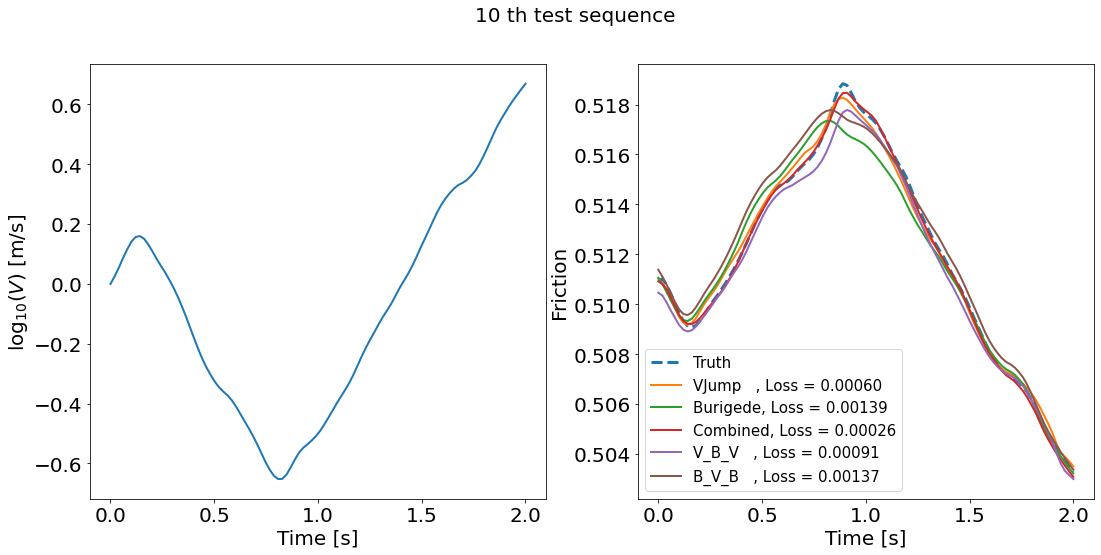
\includegraphics[width=1.0\textwidth]{./images/Trial0112_Burigede10.png}
\end{figure}
\begin{figure}[H]
    \centering
    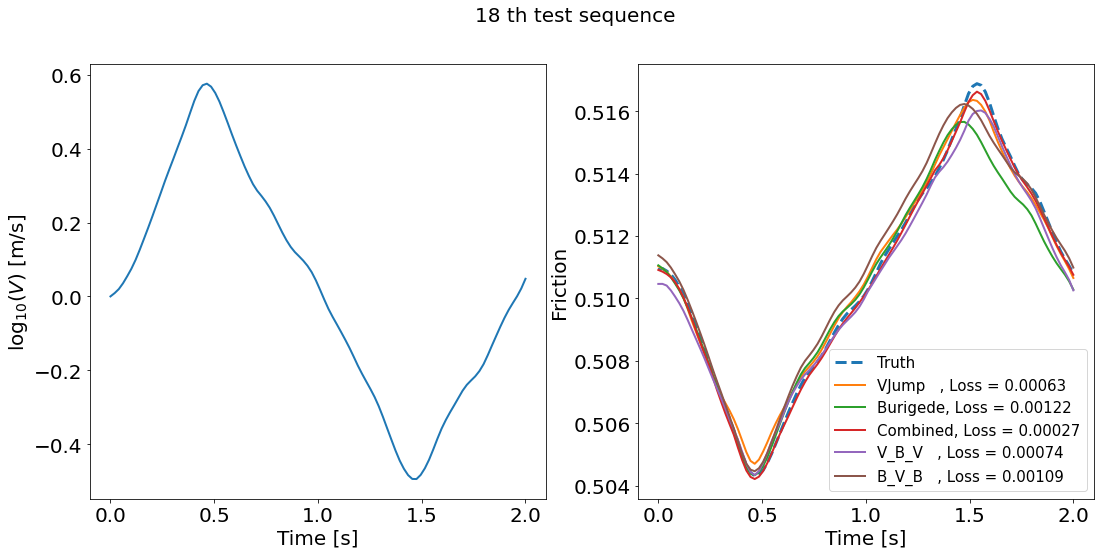
\includegraphics[width=1.0\textwidth]{./images/Trial0112_Burigede18.png}
\end{figure}
\begin{figure}[H]
    \centering
    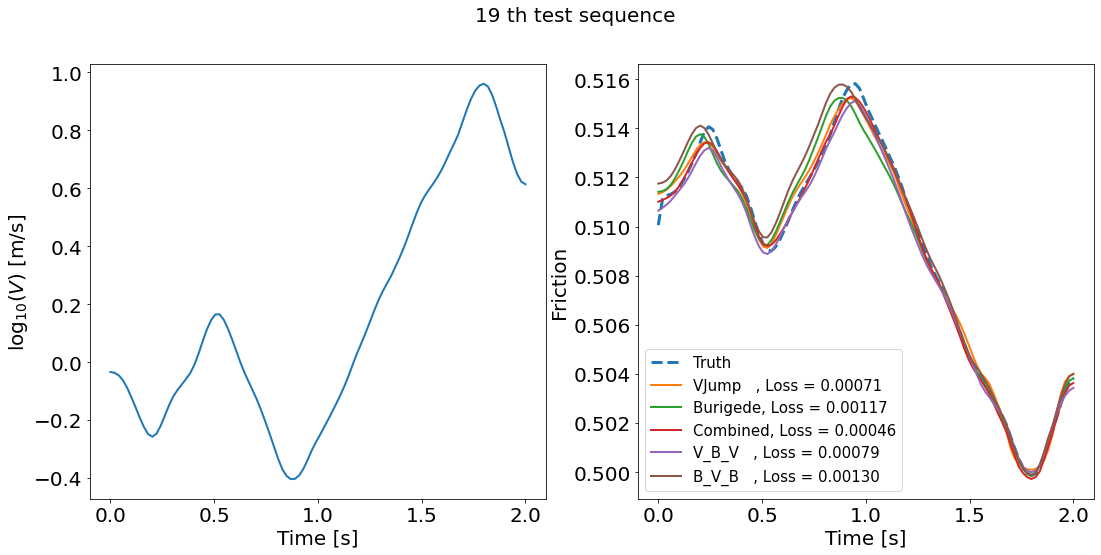
\includegraphics[width=1.0\textwidth]{./images/Trial0112_Burigede19.png}
\end{figure}

\newpage
\subsection{Plots of potentials}
From the best-fitting model (combined\textunderscore full as in Tables~\ref{tab:combinedImprovesPerformance}, \ref{tab:staggeredDoesNotImprovePerformance}), 
we plot the following potential functions as defined in ($\ref{eq:potentialWDDotX}, \ref{eq:potentialDDotX})$ (also repeated here):
\begin{align*}
    F_{fric}(\dot{x}, \boldsymbol{\xi}) &= \frac{\partial W}{\partial x}(x) + \frac{\partial D^\dagger}{\partial \dot{x}}(\dot{x}, \bm{\xi}),\\
    \frac{d D}{d \dot{\boldsymbol{\xi}}} + \frac{\partial D^\dagger}{\partial \boldsymbol{\xi}} &= 0.
\end{align*}
The red dots represent the data points in the training dataset. 

\begin{figure}[H]
    \centering
    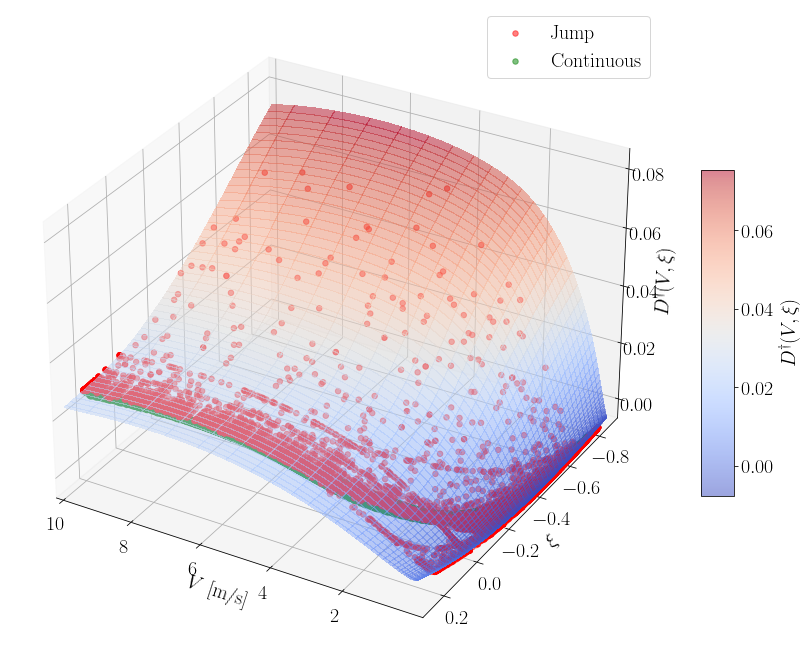
\includegraphics[width=0.7\textwidth]{images/Trial0216_combined_800_D_dagger_normal.png}
    \caption{$D^\dagger(\dot{x}, \xi)$: $\mathbb{R}\times\mathbb{R}\rightarrow \mathbb{R}$}
    \label{fig:DDaggerPlot}
\end{figure}
The learnt $D^\dagger$ is not convex. 
Moreover, 
it seems to be concave in $V=\dot{x}$ but convex in $\xi$ for any given $(\dot{x}, \xi)$. 

\begin{figure}[H]
    \centering
    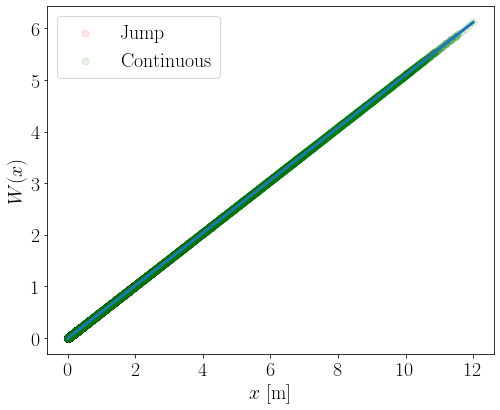
\includegraphics[width=0.5\textwidth]{images/Trial0216_combined_800_W.png}
    \caption{$W(x)$: $\mathbb{R}\rightarrow \mathbb{R}$}
    \label{fig:WPlot}
\end{figure}
The learnt $W(x)$ is non-convex. 

\begin{figure}[H]
    \centering
    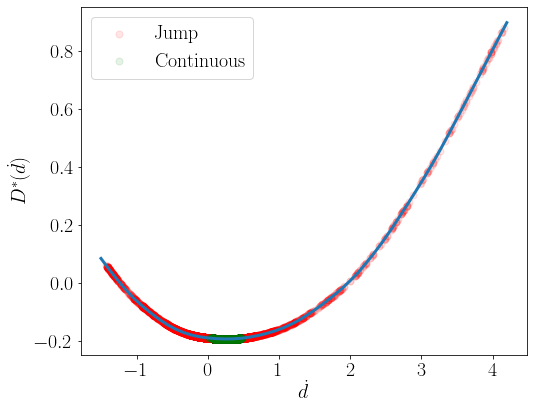
\includegraphics[width=0.5\textwidth]{images/Trial0216_combined_800_D_star.png}
    \caption{$D^*(\dot{d})$: $\mathbb{R}\rightarrow \mathbb{R}$}
    \label{fig:DStarPlot}
\end{figure}
The learnt $D^*$ is convex, 
and thus we can find $d(\dot{\bm{\xi}})$ in that region.  

Another thing we noticed is that
\textbf{the VJump dataset explores a larger domain in the phase space compared to the Burigede dataset}, 
which can be seen from Figure~\ref{fig:DDaggerPlot} especially. 

\newpage
\subsubsection{Non-uniqueness of $\xi$}
\begin{figure}[H]
    \centering
    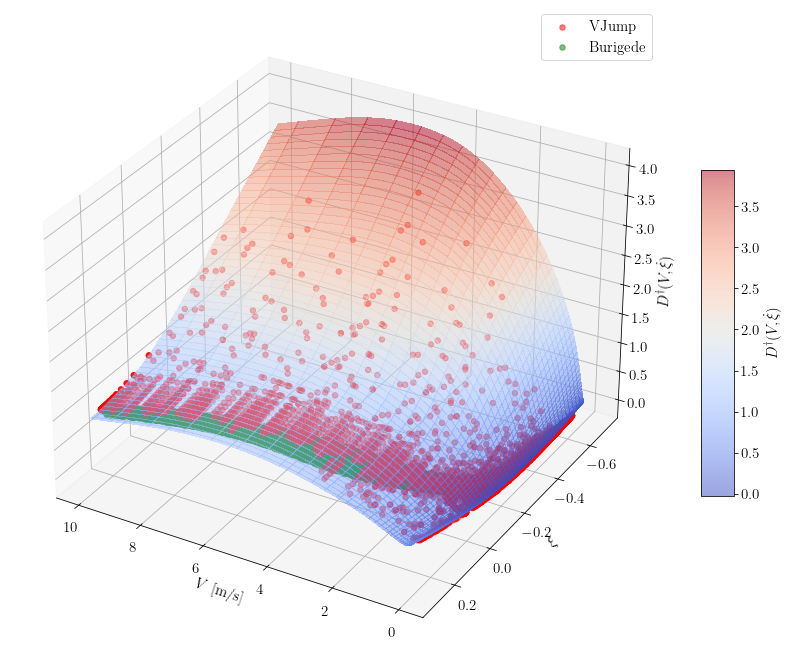
\includegraphics[width=0.4\textwidth]{images/Trial0112_combined_D_dagger_normal.png}
    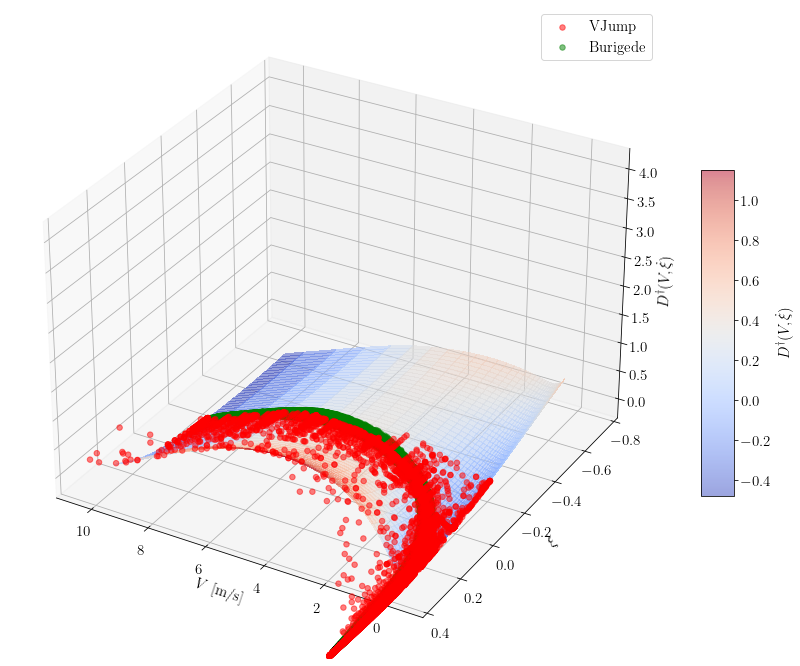
\includegraphics[width=0.4\textwidth]{images/Trial0112_smallA_smallDRS_D_dagger_normal.png}
    \caption{$D^\dagger(\dot{x}, \xi)$: $\mathbb{R}\times\mathbb{R}\rightarrow \mathbb{R}$ trained on combined (left) and VJump only (right) datasets}
    \label{fig:DDaggerPlotCompare}
\end{figure}
\begin{figure}[H]
    \centering
    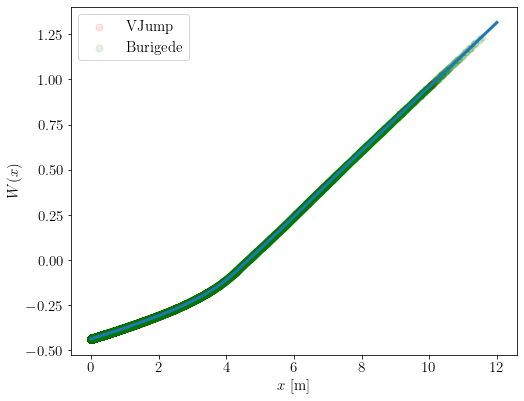
\includegraphics[width=0.4\textwidth]{images/Trial0112_combined_W.png}
    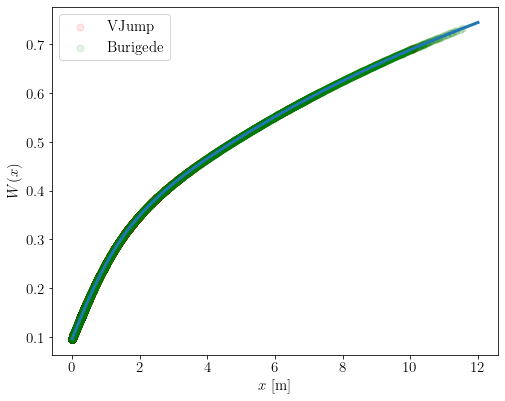
\includegraphics[width=0.4\textwidth]{images/Trial0112_smallA_smallDRS_W.png}
    \caption{$W(x)$: $\mathbb{R} \rightarrow \mathbb{R}$ trained on combined (left) and VJump only (right) datasets}
    \label{fig:DDaggerPlotCompare}
\end{figure}
\begin{figure}[H]
    \centering
    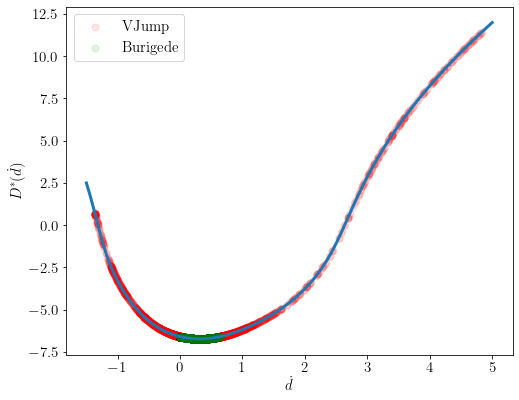
\includegraphics[width=0.4\textwidth]{images/Trial0112_combined_D_star.png}
    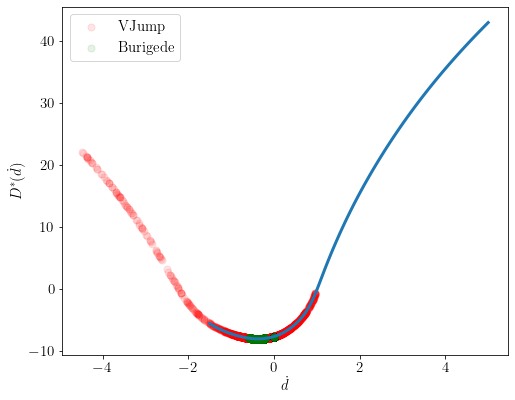
\includegraphics[width=0.4\textwidth]{images/Trial0112_smallA_smallDRS_D_star.png}
    \caption{$D^*(\dot{d})$: $\mathbb{R}\rightarrow \mathbb{R}$ trained on combined (left) and VJump only (right) datasets}
    \label{fig:DDaggerPlotCompare}
\end{figure}

% Check that different $\xi$s are different by a linear map
\subsubsection{$\xi$'s are invariant up to affine maps}
We check that since $D(\dot{\bm{\xi}})$ has only one argument, i.e., $\dot{\bm{\xi}}$, 
different trained models will result in the same $\xi$ up to affine maps. 

\begin{figure}[H]
    \centering
    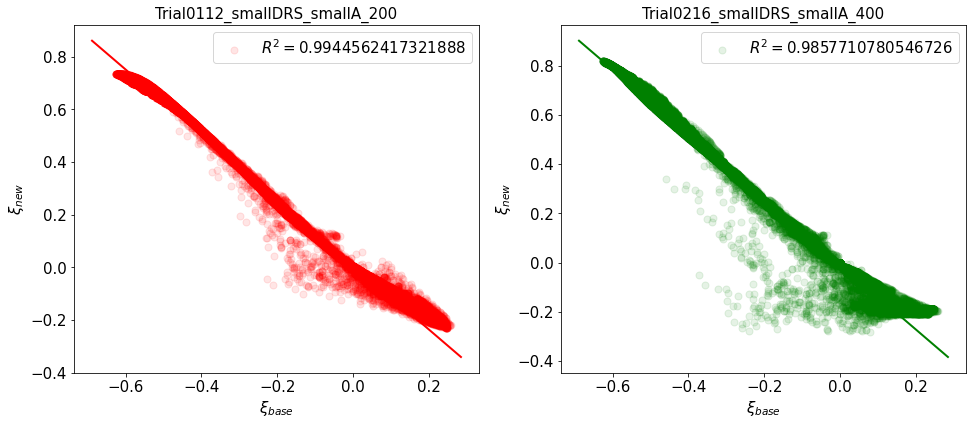
\includegraphics[width=1.0\textwidth]{images/LinReg_Xis.png}
    \caption{The $\xi$'s calculated from different trained-models are highly linearly-correlated. 
    The base model here is Trial0112_combined_400.}
    \label{fig:LinRegXis}
\end{figure}
\begin{figure}[H]
    \centering
    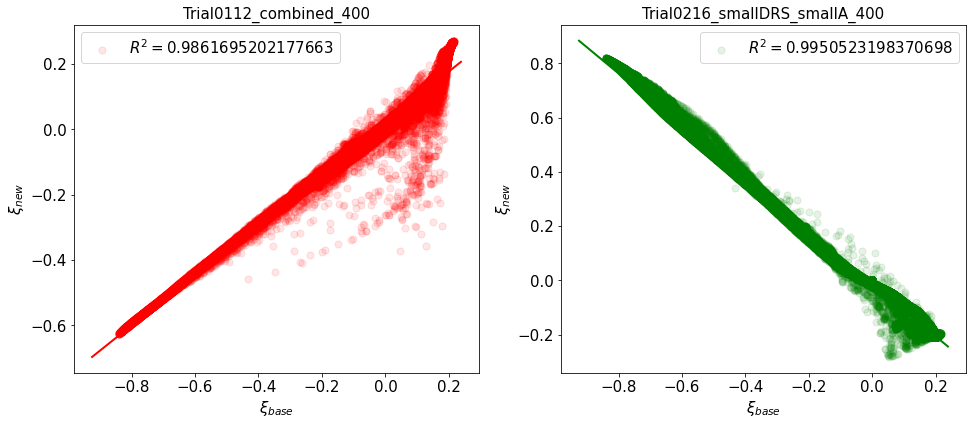
\includegraphics[width=1.0\textwidth]{images/LinReg_Xis_400_on_800.png}
    \caption{The $\xi$'s calculated from different trained-models are highly linearly-correlated. 
    The base model here is Trial0216_combined_800.}
    \label{fig:LinRegXis400On800}
\end{figure}

\subsubsection{Distribution of $\xi$'s and $-\partial D^\dagger / \partial \xi$ for velocity-jump and continuous-variation datasets.}
In this part, 
we fix the trained model to be the one trained on the combined dataset of $200$ velocity-jump sequences and $200$ continuous-variation sequences. 
Then we have consistent definition of $\xi$, 
as $\xi$'s in different trained models can be different by affine maps. 

Then we compare the distribution of $\xi$'s of different training datasets in the plot below:
\begin{figure}[H]
    \centering
    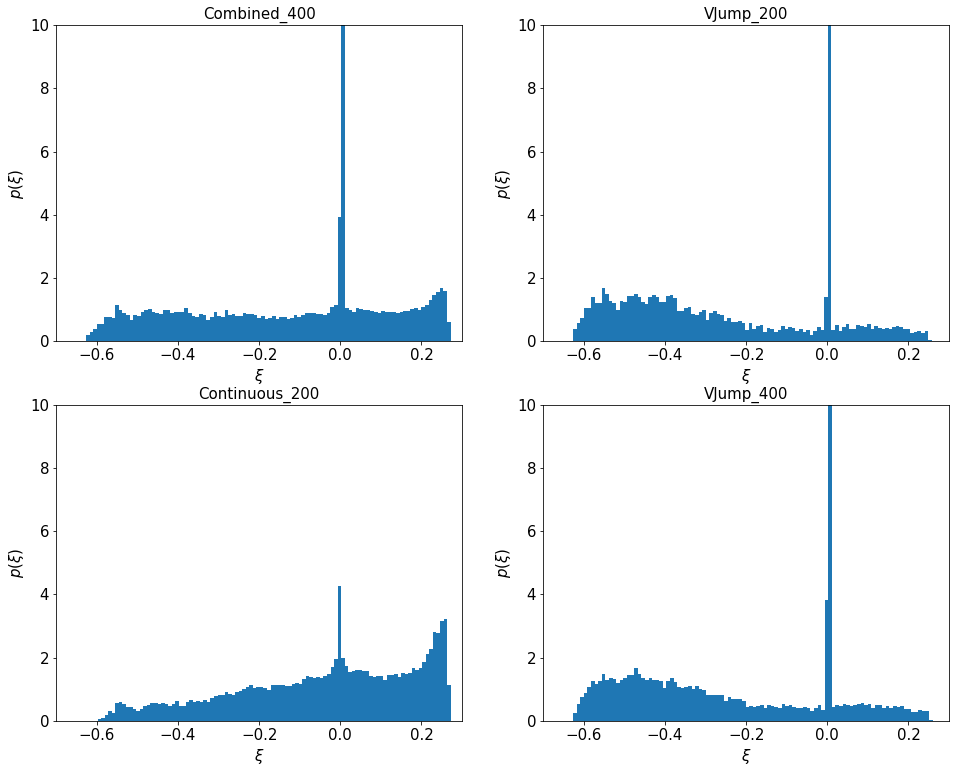
\includegraphics[width=1.0\textwidth]{images/Distri_Xis.png}
    \caption{The distribution of $\xi$'s calculated from Velocity-Jump or Continuous-Variation datasets.}
    \label{fig:DistriXis}
\end{figure}

\begin{figure}[H]
    \centering
    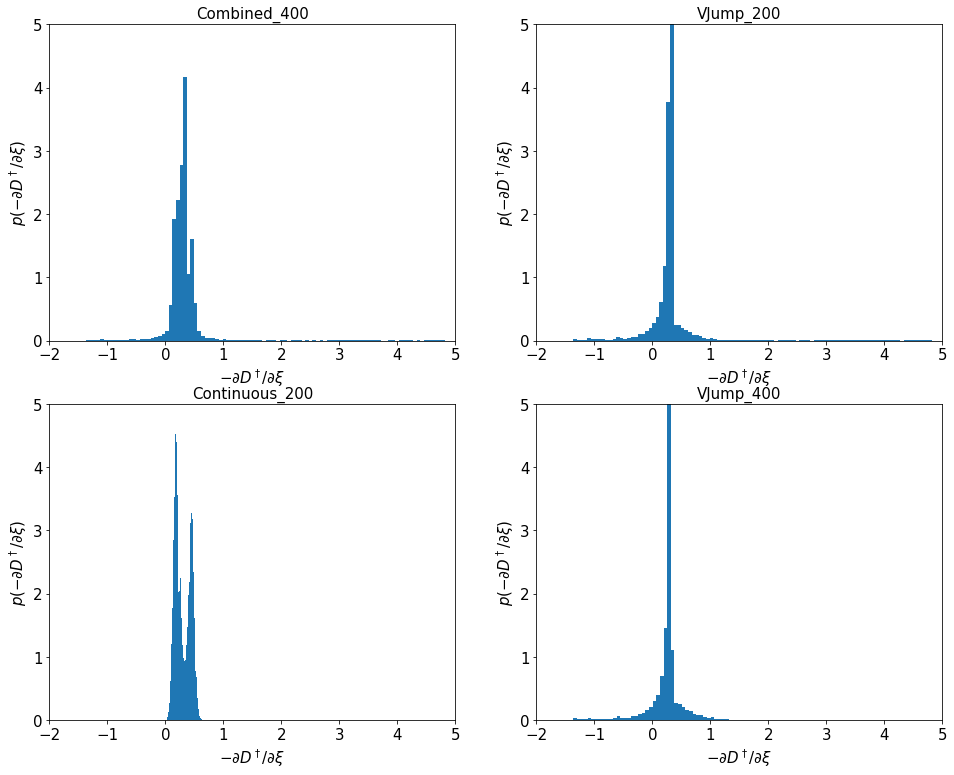
\includegraphics[width=1.0\textwidth]{images/Distri_Dins.png}
    \caption{The distribution of $-\partial D^\dagger / \partial \xi$'s calculated from Velocity-Jump or Continuous-Variation datasets.}
    \label{fig:DistriDins}
\end{figure}

\newpage
\subsection{Trained-NN to solve for spring-slider problems}
Here we use a learnt-NN to solve for spring-slider problems as posed by (\ref{eq:motion}). 
We fix the initial condition to be $\theta=0.01\ \mathrm{s}$ for rate-and-state formulation, 
and set $\xi=0$ for the trained-NN model. 
Then we generate $200$ trajectories of prescribed history:
\begin{align*}
    \{x_p(t) : t\in [0, T]\}, 
\end{align*}
the average relative $L_2$ errors of the trained-NN model against the rate-and-state model are reported in this table:
\begin{table}[H]
    \centering
    \begin{tabular}{ccc}
        \hline
        Err($x(t)$) & Err($V(t)$) & Err($f(t)$) (scaled) \\
        $(5.758 \pm 6.353) \times 10^{-5}$ & 0.0017 $\pm$ 0.0018
        & 0.064 $\pm$ 0.036\\
        \hline
    \end{tabular}
    \caption{Relative $L_2$ error in $x(t), V(t), f(t)$ averaged  over 200 sequences.}
    \label{tab:L2ErrorSpringSlider}
\end{table}
\begin{figure}[H]
    \centering
    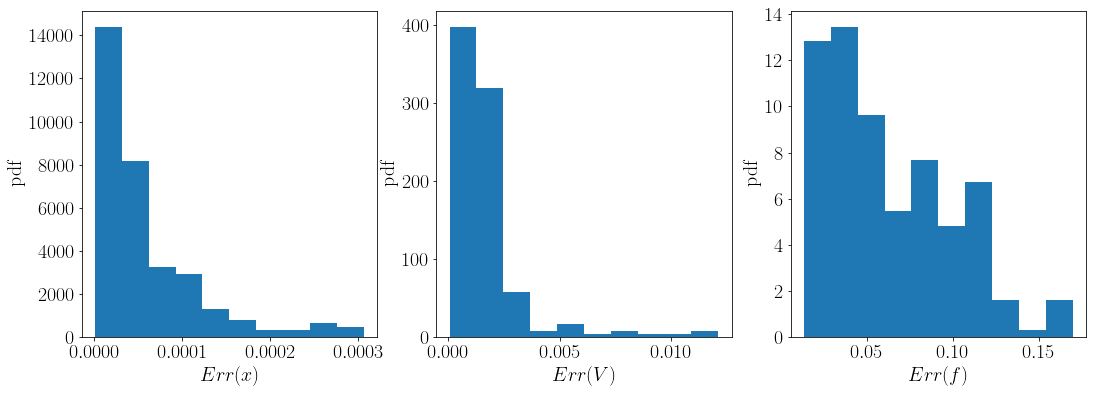
\includegraphics[width=1.0\textwidth]{images/SpringSlider_Err_XVF_pdfs.png}
    \caption{Histograms of error distributions of $x$, $V$ and $f$.}
    \label{fig:SpringSliderErrXVFPdfs}
\end{figure}
Here are a few example sequences:
\begin{figure}[H]
    \centering
    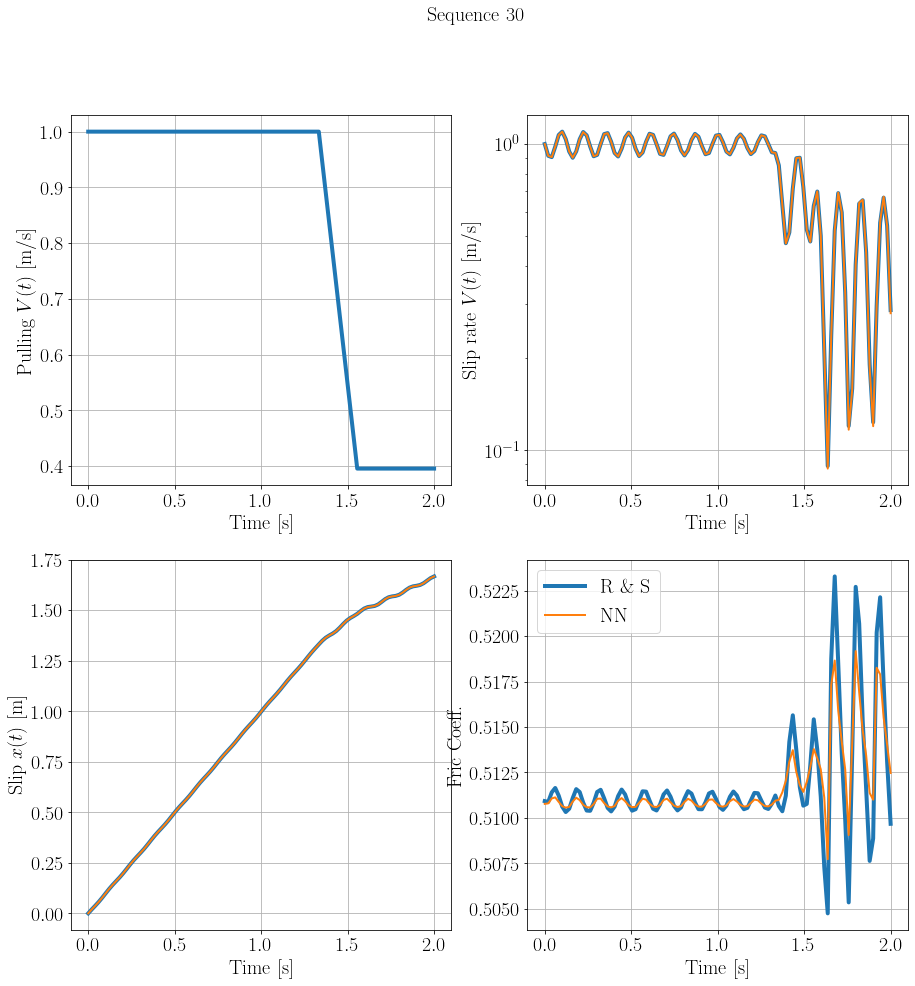
\includegraphics[width=1.0\textwidth]{images/SpringSlider30.png}
\end{figure}
\begin{figure}[H]
    \centering
    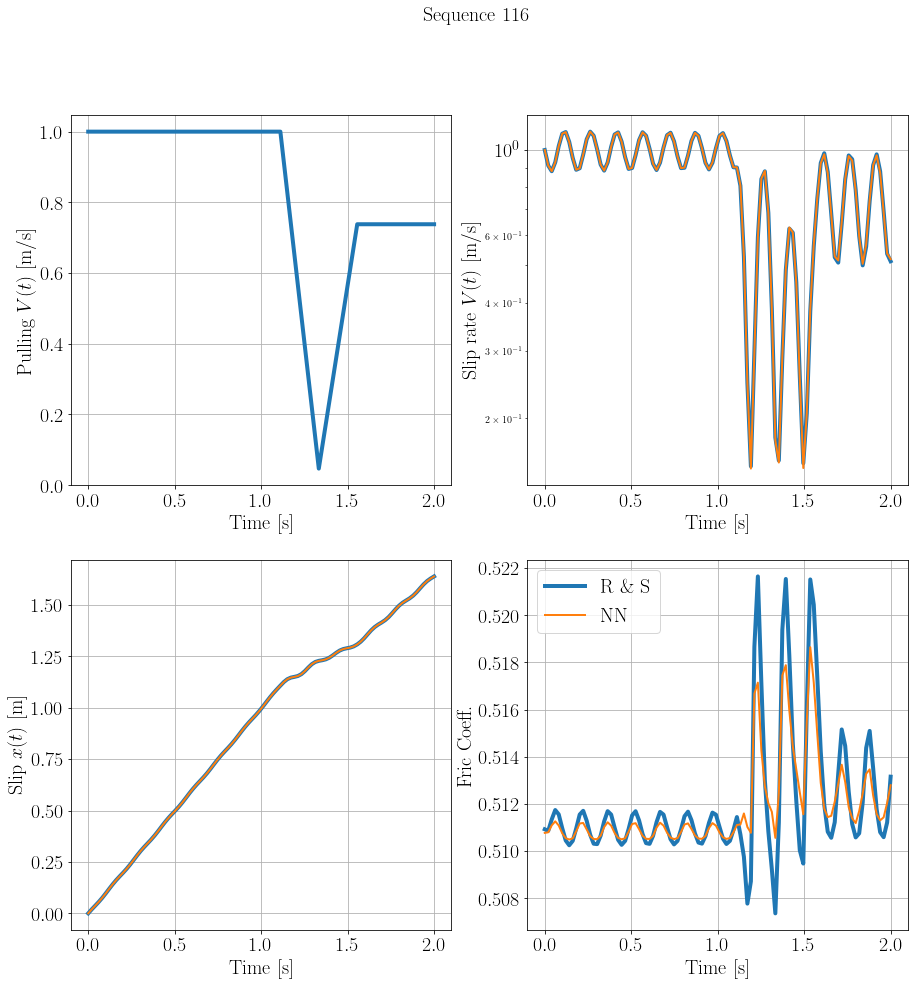
\includegraphics[width=1.0\textwidth]{images/SpringSlider116.png}
\end{figure}
\begin{figure}[H]
    \centering
    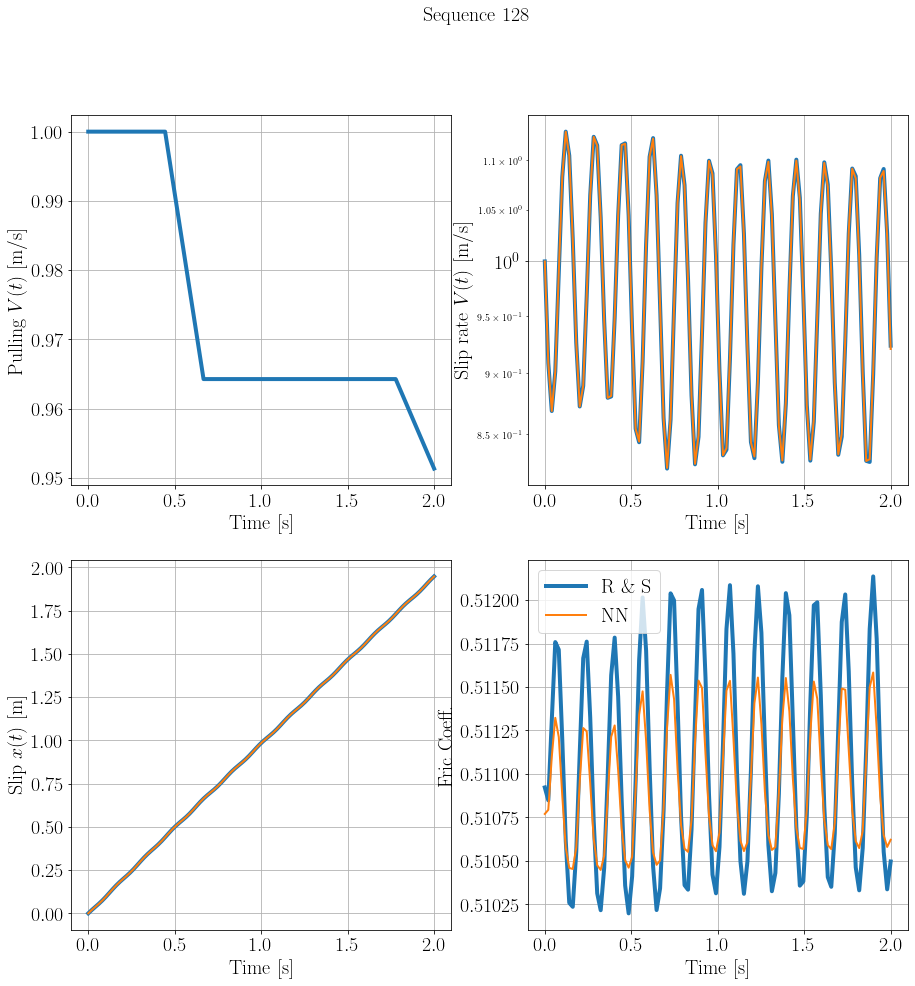
\includegraphics[width=1.0\textwidth]{images/SpringSlider128.png}
\end{figure}

\newpage
\subsection{Err vs. time step for NN and RS formulations}
In this part, 
we try to solve for the above-mentioned spring-slider model with NN and original rate and state formulations. 
We use 4th order Runge-Kutta method for explicit solve, 
and Adams method for implicit solve. 

Since we cannot obtain the true solution, 
for each (model, solver) pair, 
we first use a fine $\Delta t = 2^{-12}\ \mathrm{s}$ to solve for $V(t)$, 
and consider that to be $V_{true}(t)$. 
Relative $L_2$ errors in time are computed for each (model, solver) pair, 
for $\Delta t \in \{2^{-13.5}, 2^{-13}, 2^{-12.5}, 2^{-12}, 2^{-11.5}, 2^{-11}\}\ \mathrm{s}$. 

For sequences with relative $L_2$ errors greater than $0.2$, 
we consider that to be a wrong solution, 
which usually is because of either numerical oscillations, 
or non-converging implicit solves which results in ``NaN". 

Here we randomly sampled \textbf{200} sequences with different $k/m$ ratio for the spring slider system and different loading history $x_p(t), t \in [0, 0.5] s$, 
and try to simulate their $x(t)$'s. 
\subsubsection{Error w.r.t repective finest discretization}
\begin{figure}[H]
    \centering
    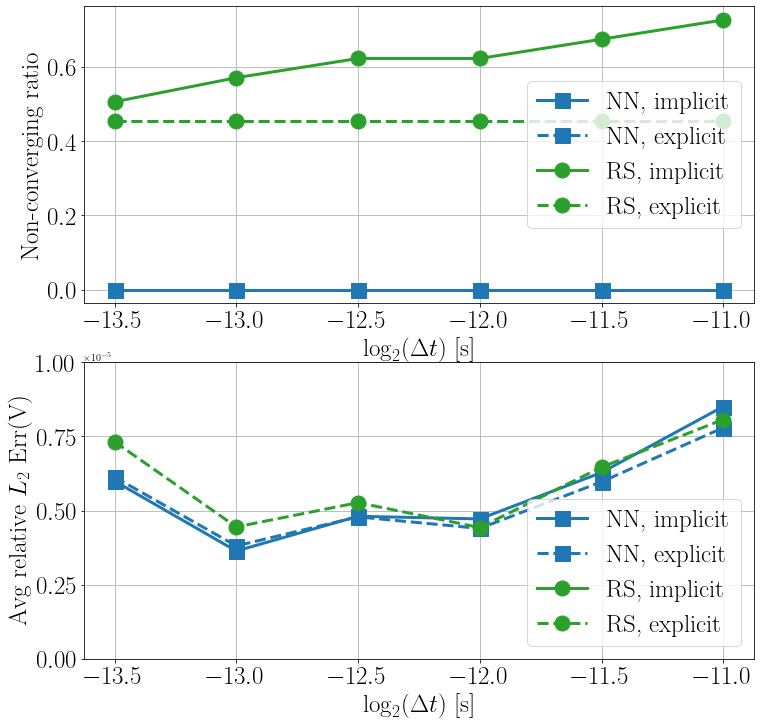
\includegraphics[width=0.7\textwidth]{images/err_timesteps_rs_nn_0531_respective.png}
\end{figure}
\begin{table}[H]
    \centering
    \begin{tabular}{cccccccc}
        \hline
        $\Delta t$ [s] & $2^{-13.5}$ & $2^{-13.0}$ & $2^{-12.5}$ & $2^{-12.0}$ & $2^{-11.5}$ & $2^{-11.0}$ \\
        \hline
        NN, implicit & 0.000 & 0.000 & 0.000 & 0.000 & 0.000 & 0.000 \\
        NN, explicit & 0.000 & 0.000 & 0.000 & 0.000 & 0.000 & 0.000 \\
        RS, implicit & 0.506 & 0.571 & 0.623 & 0.623 & 0.675 & 0.727 \\
        RS, explicit & 0.455 & 0.455 & 0.455 & 0.455 & 0.455 & 0.455 \\
        \hline
    \end{tabular}
    \caption{Ratio of sequences with relative $L_2$ error larger than $0.2$,  
    for NN, RS models with implicit, explicit solvers.}
    \label{tab:NaNRatioSpringSliderRsVsNNRespective}
\end{table}

\begin{table}[H]
    \centering
    \begin{tabular}{ccccccc}
        \hline
        $\Delta t$ [s] & $2^{-13.5}$ & $2^{-13.0}$ & $2^{-12.5}$ & $2^{-12.0}$ & $2^{-11.5}$ & $2^{-11.0}$ \\
        \hline
        NN, implicit & 5.993e-06 & 3.636e-06 & 4.807e-06 & 4.716e-06 & 6.282e-06 & 8.508e-06 \\
        NN, explicit & 6.130e-06 & 3.808e-06 & 4.786e-06 & 4.397e-06 & 5.968e-06 & 7.795e-06 \\
        RS, implicit & nan & nan & nan & nan & nan & nan \\
        RS, explicit & 7.321e-06 & 4.447e-06 & 5.267e-06 & 4.426e-06 & 6.464e-06 & 8.069e-06 \\
        \hline
    \end{tabular}
    \caption{Mean relative $L_2$ error in $V(t)$ averaged over 200 sequences, 
    for NN, RS models with implicit, explicit solvers.}
    \label{tab:MeanL2ErrorSpringSliderRsVsNNRespective}
\end{table}

\begin{table}[H]
    \centering
    \begin{tabular}{cccccccc}
        \hline
        $\Delta t$ [s] & $2^{-13.5}$ & $2^{-13.0}$ & $2^{-12.5}$ & $2^{-12.0}$ & $2^{-11.5}$ & $2^{-11.0}$ \\
        \hline
        NN, implicit & 5.799e-06 & 5.390e-06 & 5.575e-06 & 7.069e-06 & 6.384e-06 & 1.033e-05 \\
        NN, explicit & 6.241e-06 & 5.766e-06 & 5.844e-06 & 6.887e-06 & 6.572e-06 & 9.639e-06 \\
        RS, implicit & nan & nan & nan & nan & nan & nan \\
        RS, explicit & 9.601e-06 & 6.886e-06 & 5.541e-06 & 5.597e-06 & 6.845e-06 & 1.017e-05 \\
        \hline
    \end{tabular}
    \caption{Standard deviation of relative $L_2$ error in $V(t)$ over 200 sequences, 
    for NN, RS models with implicit, explicit solvers.}
    \label{tab:StdL2ErrorSpringSliderRsVsNNRespective}
\end{table}
\subsubsection{Error w.r.t repective finest discretization}
\begin{figure}[H]
    \centering
    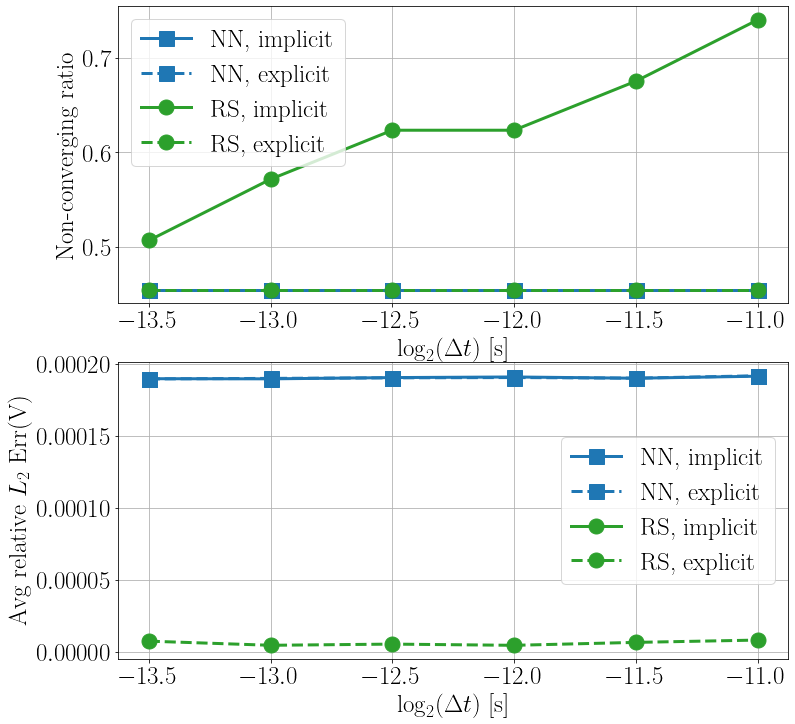
\includegraphics[width=0.7\textwidth]{images/err_timesteps_rs_nn_0531_universal.png}
\end{figure}
\begin{table}[H]
    \centering
    \begin{tabular}{cccccccc}
        \hline
        $\Delta t$ [s] & $2^{-13.5}$ & $2^{-13.0}$ & $2^{-12.5}$ & $2^{-12.0}$ & $2^{-11.5}$ & $2^{-11.0}$ \\
        \hline
        NN, implicit & 0.000 & 0.000 & 0.000 & 0.000 & 0.000 & 0.000 \\
        NN, explicit & 0.000 & 0.000 & 0.000 & 0.000 & 0.000 & 0.000 \\
        RS, implicit & 0.506 & 0.571 & 0.623 & 0.623 & 0.675 & 0.727 \\
        RS, explicit & 0.455 & 0.455 & 0.455 & 0.455 & 0.455 & 0.455 \\
        \hline
    \end{tabular}
    \caption{Ratio of sequences with relative $L_2$ error larger than $0.2$,  
    for NN, RS models with implicit, explicit solvers.}
    \label{tab:NaNRatioSpringSliderRsVsNNUniversal}
\end{table}

\begin{table}[H]
    \centering
    \begin{tabular}{ccccccc}
        \hline
        $\Delta t$ [s] & $2^{-13.5}$ & $2^{-13.0}$ & $2^{-12.5}$ & $2^{-12.0}$ & $2^{-11.5}$ & $2^{-11.0}$ \\
        \hline
        NN, implicit & 1.896e-04 & 1.895e-04 & 1.904e-04 & 1.908e-04 & 1.899e-04 & 1.913e-04 \\
        NN, explicit & 1.894e-04 & 1.898e-04 & 1.902e-04 & 1.904e-04 & 1.900e-04 & 1.916e-04 \\
        RS, implicit & nan & nan & nan & nan & nan & nan \\
        RS, explicit & 7.321e-06 & 4.447e-06 & 5.267e-06 & 4.426e-06 & 6.464e-06 & 8.069e-06 \\
        \hline
    \end{tabular}
    \caption{Mean relative $L_2$ error in $V(t)$ averaged over 200 sequences, 
    for NN, RS models with implicit, explicit solvers.}
    \label{tab:MeanL2ErrorSpringSliderRsVsNNUniversal}
\end{table}

\begin{table}[H]
    \centering
    \begin{tabular}{cccccccc}
        \hline
        $\Delta t$ [s] & $2^{-13.5}$ & $2^{-13.0}$ & $2^{-12.5}$ & $2^{-12.0}$ & $2^{-11.5}$ & $2^{-11.0}$ \\
        \hline
        NN, implicit & 4.535e-04 & 4.530e-04 & 4.536e-04 & 4.537e-04 & 4.530e-04 & 4.530e-04 \\
        NN, explicit & 4.532e-04 & 4.533e-04 & 4.536e-04 & 4.537e-04 & 4.534e-04 & 4.525e-04 \\
        RS, implicit & nan & nan & nan & nan & nan & nan \\
        RS, explicit & 9.601e-06 & 6.886e-06 & 5.541e-06 & 5.597e-06 & 6.845e-06 & 1.017e-05 \\
        \hline
    \end{tabular}
    \caption{Standard deviation of relative $L_2$ error in $V(t)$ over 200 sequences, 
    for NN, RS models with implicit, explicit solvers.}
    \label{tab:StdL2ErrorSpringSliderRsVsNNUniversal}
\end{table}

\newpage
\subsection{Using Polynomials to fit the learnt NN potentials}
Here I try to use polynomials (with order $\le 4$) as the basis functions for the potentials, i.e., 
assuming 
\begin{align*}
    W(x) &= w_0 + w_1 x + w_2 x^2 + w_3 x^3 + ... \\
    D^\dagger(v, \xi) &= \left[v, v^2, \xi, \xi^2, \log(v), v\xi, 
                          v\log(v), \xi \log(v), v^2\log(v), v\log(v) \xi, 
                          \log(v)\xi^2 \right] w_{D^\dagger} + b_{D^\dagger} \\
    D^*(\dot{d}) &= d^*_0 + d^*_1 \dot{d} + d^*_2 \dot{d}^2 + d^*_3 \dot{d}^3 + d^*_4 \dot{d}^4 \\
\end{align*}
We tried this on a dataset with $800$ of a combination of velocity-jump and continuous variation trajectories. 
We linearly regress those coefficients to a uniform grid over the bounded domain of $(x, v, \xi, \dot{d})$'s and the NN outputs $(W, D, D^\dagger)$'s as observed in the dataset used for training the corresponding NNs. 
Then we initialize the coefficients of the polynomial-potentials with those regressed values, 
and try to further train those coefficients using the training trajectories (essentially the same as training NNs). 

The relative $L_2$ error of scaled $f(t)$ compared with NN-based potentials trained on the same dataset:
\begin{table}[H]
    \centering
    \begin{tabular}{c|ccc}
        \hline
        Training \& Test set & Neural Net & Regressed Polynomials & Further-trained Regressed Polys. \\
        Combined (800) & 0.0173 & 0.6393 & 0.0789 \\
        \hline
    \end{tabular}
    \caption{Test error (relative $L_2(t)$ error on scaled $f(t)$) using Neural Network vs. linearly-regressed polynomials vs. further trained linearly-regressed polynomials. }
    \label{tab:NNVsPolynomialErr}
\end{table}
The average error of Further trained Regressed Polynomials can achieve 4-5 times that of the trained NNs (0.0789 vs. 0.0173).  
\subsubsection{NN vs. Polynomial potentials}
\begin{figure}[H]
    \centering
    \subfigure[]{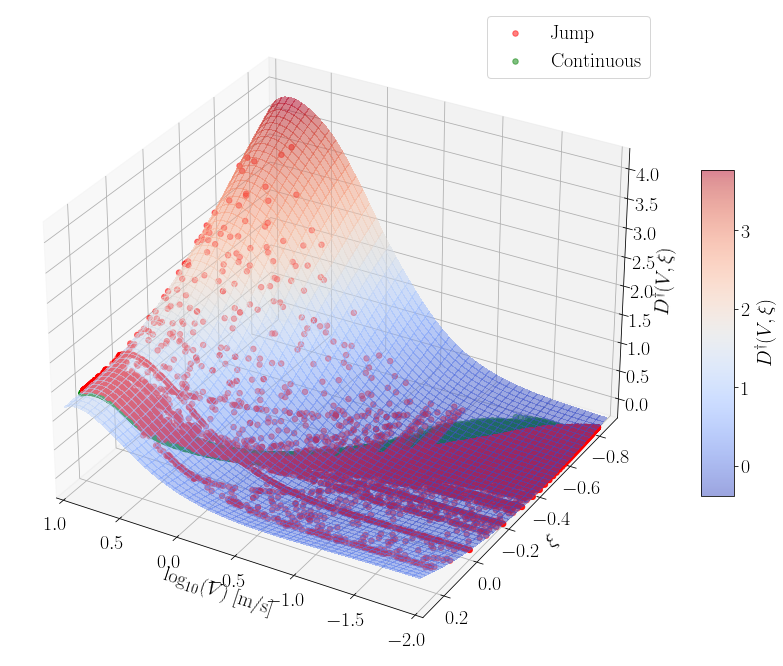
\includegraphics[width=0.48\textwidth]{images/Trial0216_combined_800_D_dagger_log.png}}
    \subfigure[]{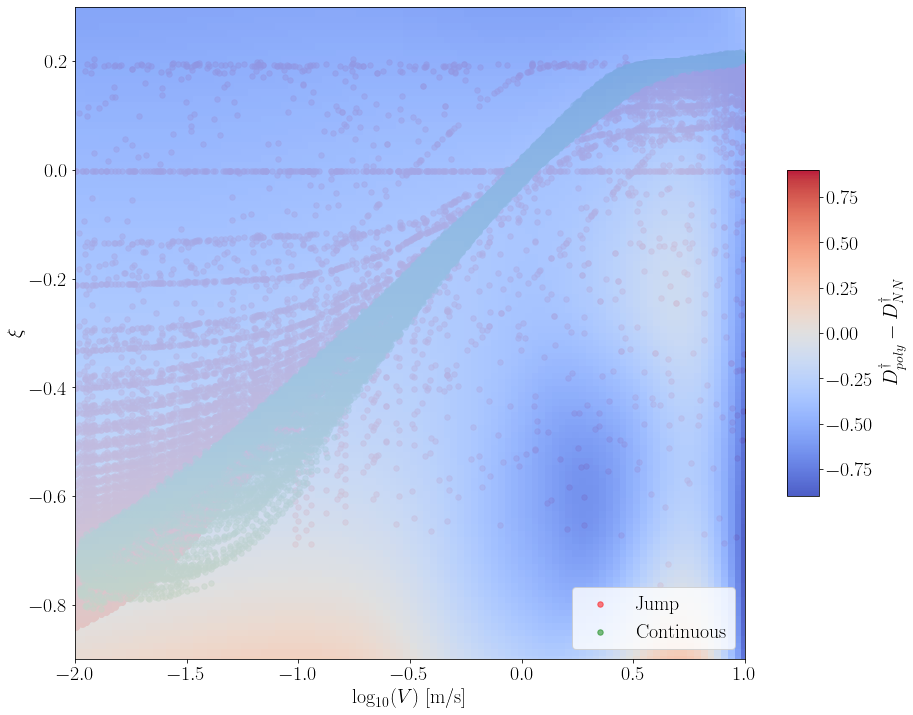
\includegraphics[width=0.48\textwidth]{images/Trial0216_combined_800_D_dagger_log_polyerr.png}}
    \caption{NN vs. polynomial $D^\dagger(\dot{x}, \xi)$}
    \label{fig:DDaggerPolyPlotCompare}
\end{figure}
\begin{figure}[H]
    \centering
    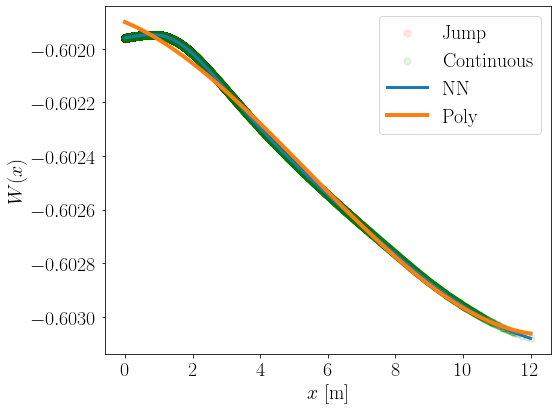
\includegraphics[width=0.7\textwidth]{images/Trial0216_combined_800_W_polyerr.png}
    \caption{NN vs. polynomial $W(x)$}
\end{figure}
\begin{figure}[H]
    \centering
    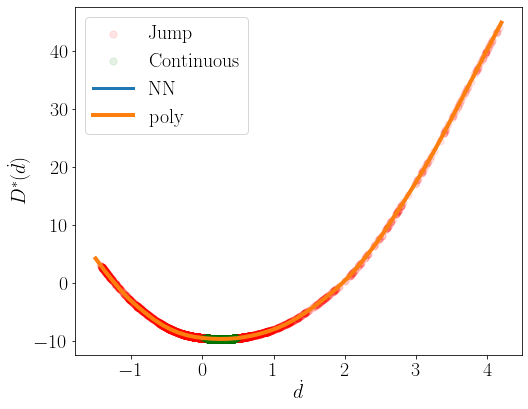
\includegraphics[width=0.7\textwidth]{images/Trial0216_combined_800_D_star_polyerr.png}
    \caption{NN vs. polynomial $D^*(\dot{d})$}
\end{figure}

\subsubsection{Specific sequences}
Here are a few fitting results by both the Neural Net and Polynomial learnt potentials:
\begin{figure}[H]
    \centering
    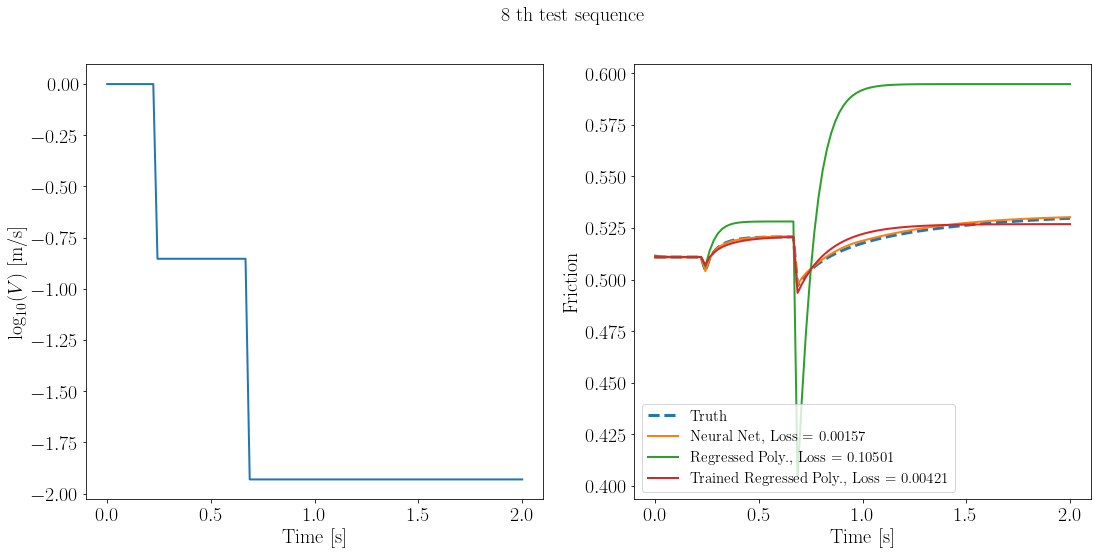
\includegraphics[width=1.0\textwidth]{images/polynomialRegressedTrainedSeq8.png}
\end{figure}
\begin{figure}[H]
    \centering
    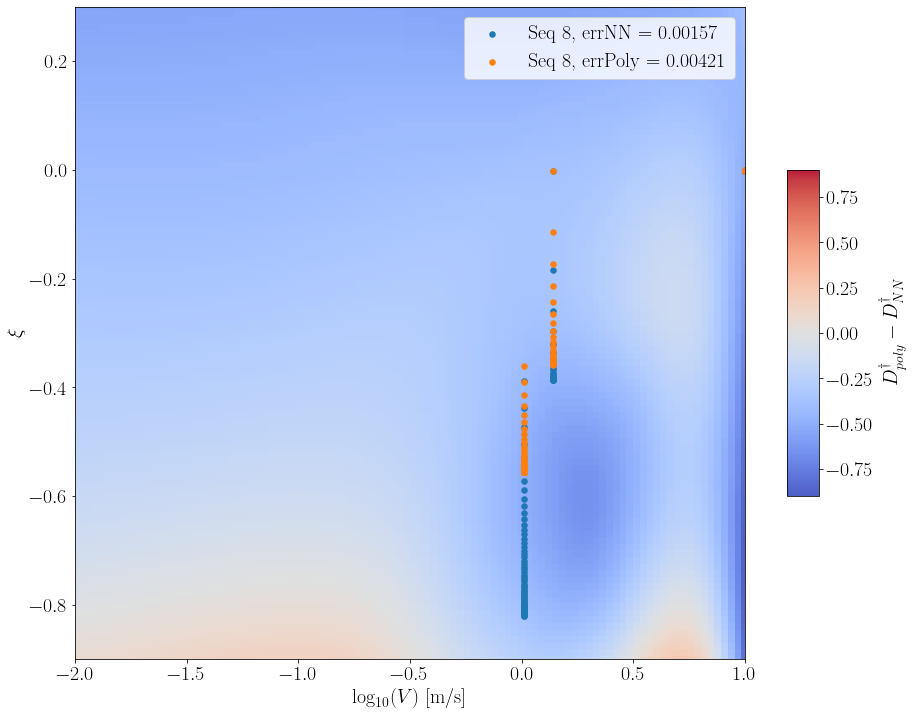
\includegraphics[width=0.7\textwidth]{images/Trial0216_errDdagger_seq8.png}
\end{figure}
\begin{figure}[H]
    \centering
    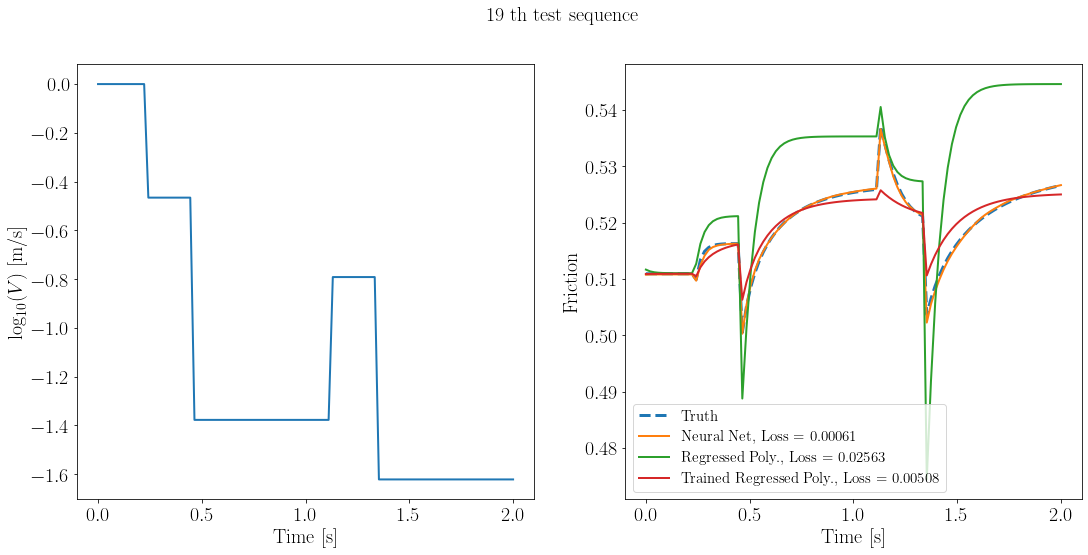
\includegraphics[width=1.0\textwidth]{images/polynomialRegressedTrainedSeq19.png}
\end{figure}
\begin{figure}[H]
    \centering
    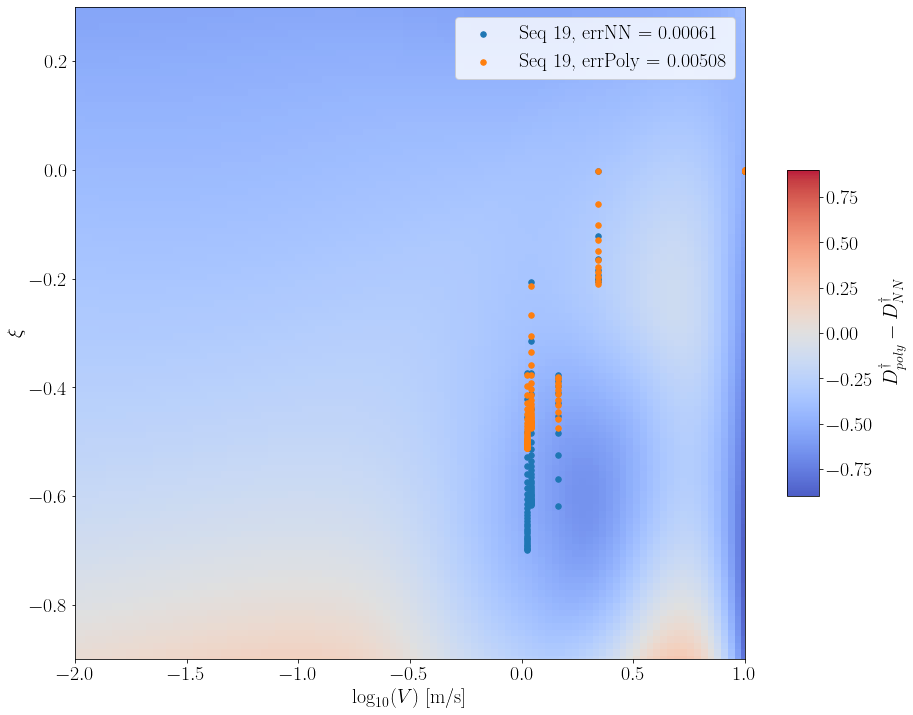
\includegraphics[width=0.7\textwidth]{images/Trial0216_errDdagger_seq19.png}
\end{figure}
\begin{figure}[H]
    \centering
    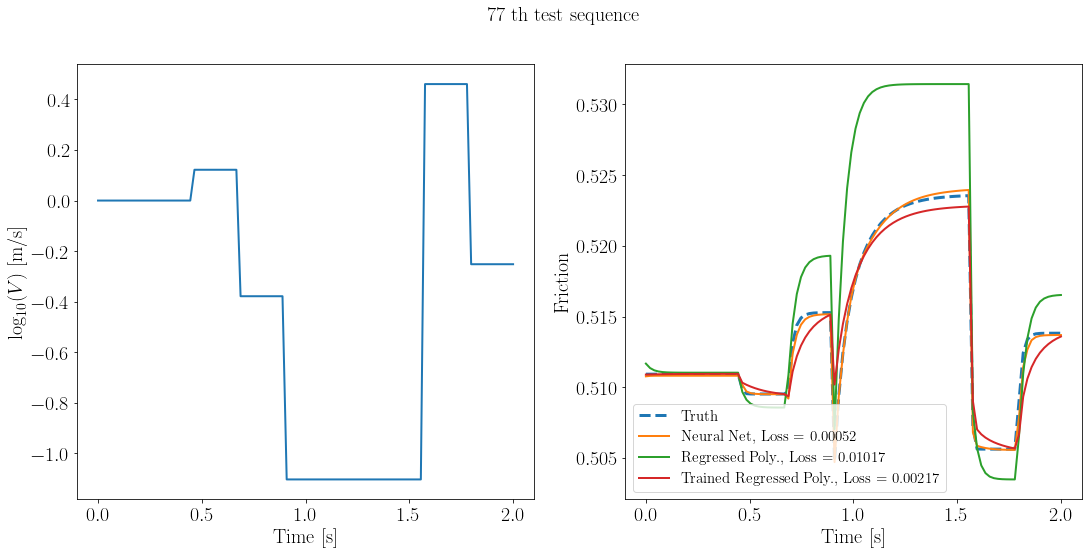
\includegraphics[width=1.0\textwidth]{images/polynomialRegressedTrainedSeq77.png}
\end{figure}
\begin{figure}[H]
    \centering
    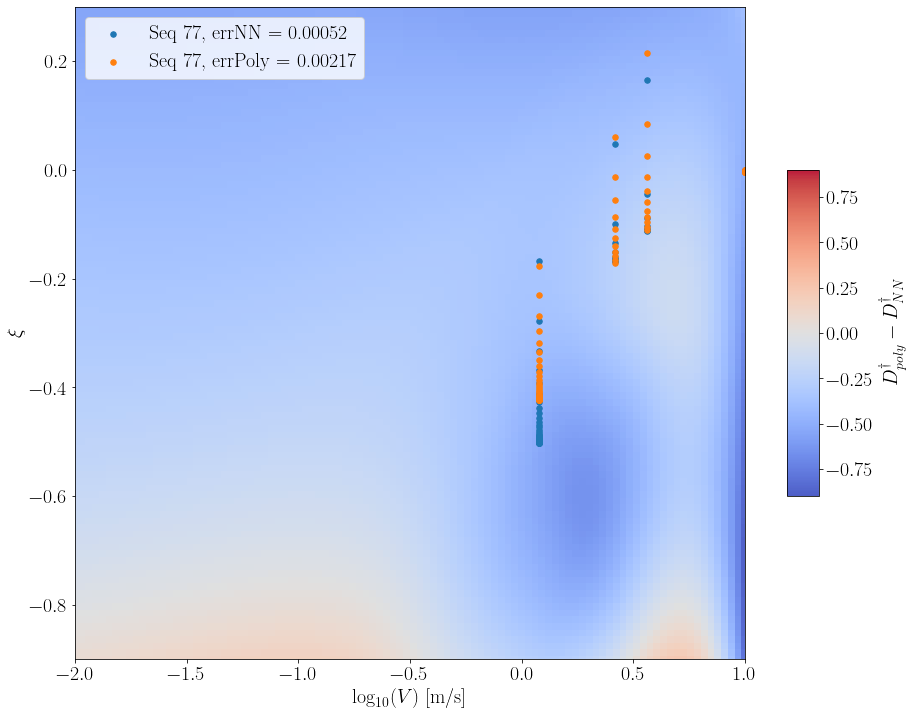
\includegraphics[width=0.7\textwidth]{images/Trial0216_errDdagger_seq77.png}
\end{figure}
\begin{figure}[H]
    \centering
    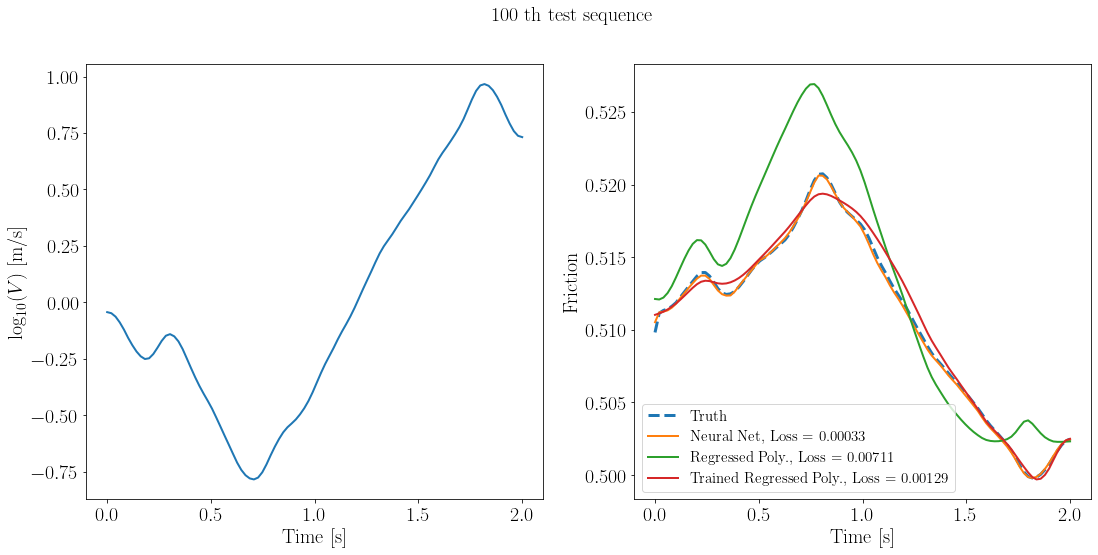
\includegraphics[width=1.0\textwidth]{images/polynomialRegressedTrainedSeq100.png}
\end{figure}
\begin{figure}[H]
    \centering
    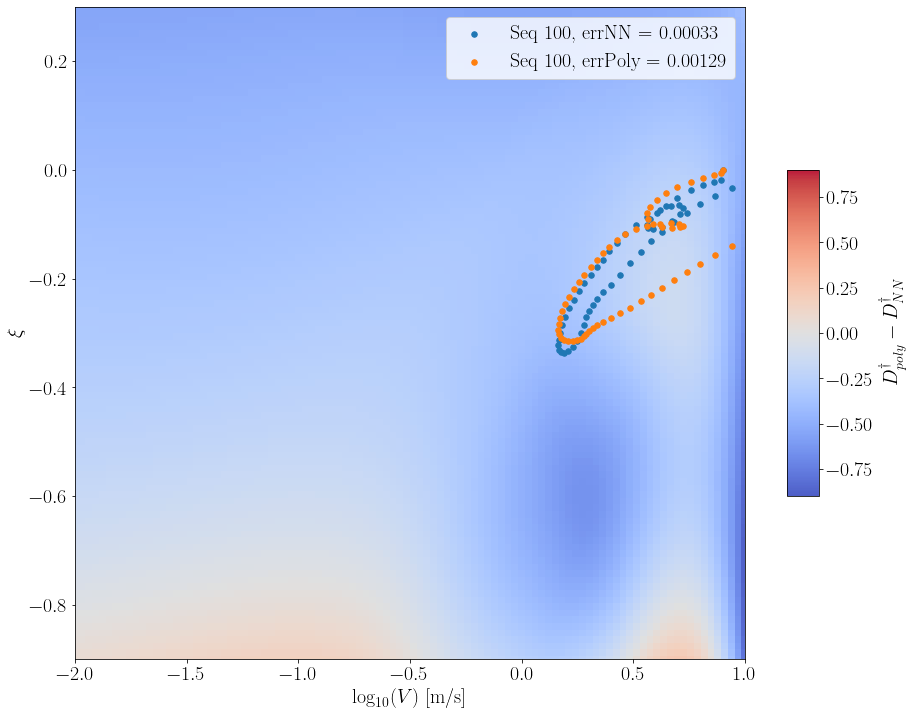
\includegraphics[width=0.7\textwidth]{images/Trial0216_errDdagger_seq100.png}
\end{figure}
\begin{figure}[H]
    \centering
    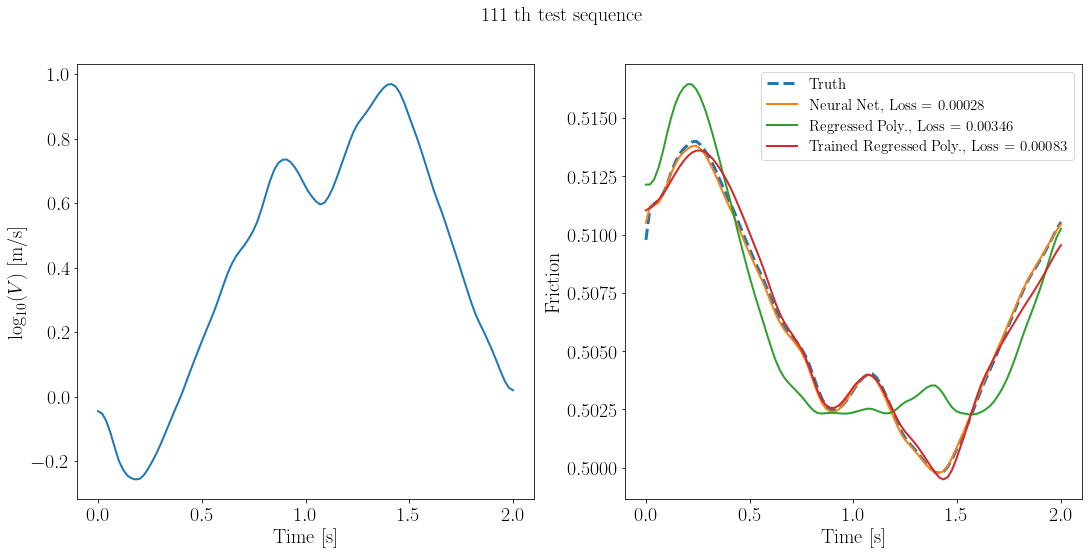
\includegraphics[width=1.0\textwidth]{images/polynomialRegressedTrainedSeq111.png}
\end{figure}
\begin{figure}[H]
    \centering
    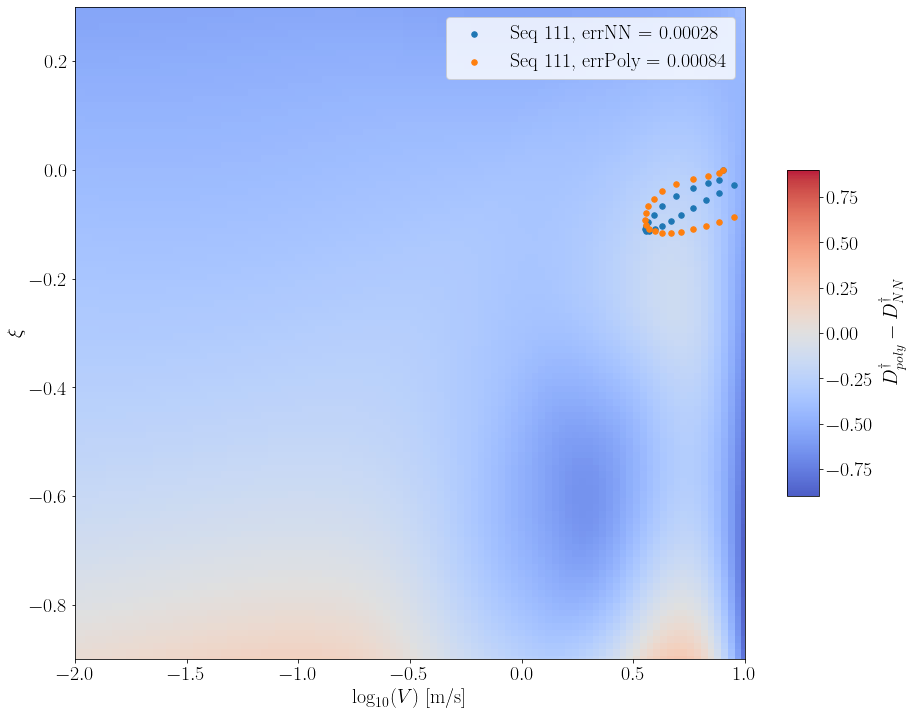
\includegraphics[width=0.7\textwidth]{images/Trial0216_errDdagger_seq111.png}
\end{figure}
\begin{figure}[H]
    \centering
    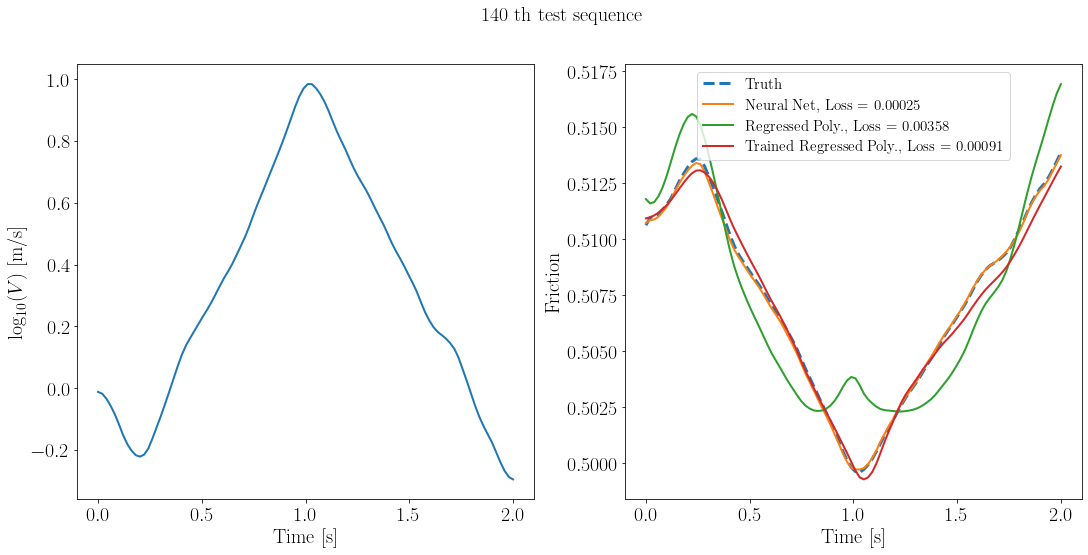
\includegraphics[width=1.0\textwidth]{images/polynomialRegressedTrainedSeq140.png}
\end{figure}
\begin{figure}[H]
    \centering
    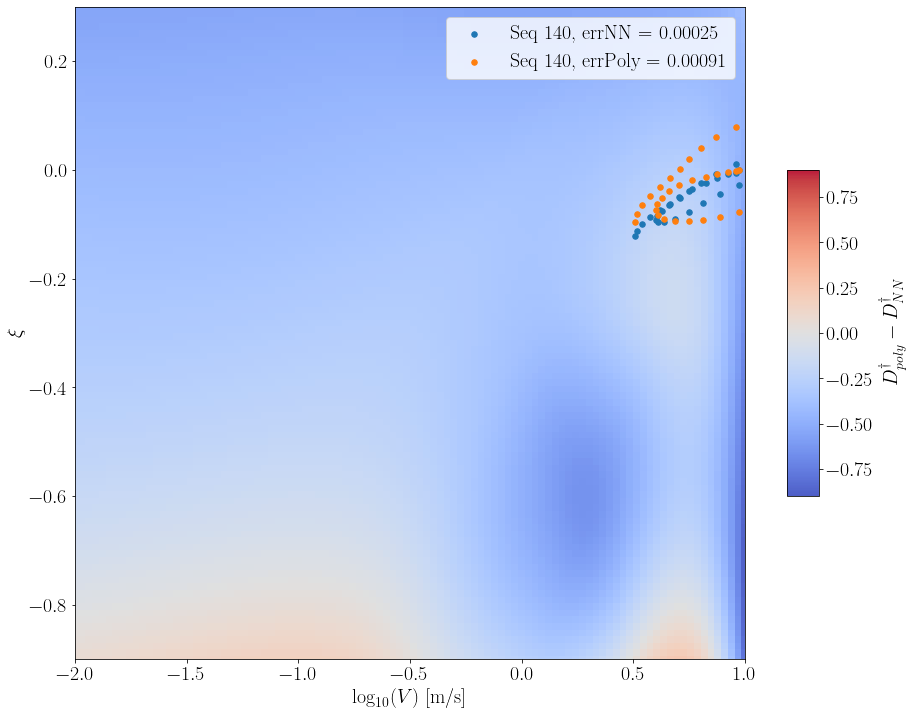
\includegraphics[width=0.7\textwidth]{images/Trial0216_errDdagger_seq140.png}
\end{figure}


\end{document}
